\chapter{Double Higgs Bosons Production Analysis}
\label{chap:DoubleHiggs}

\chapterquote{Two is better than one}%
{Sir Steve Orange, 1785--1854}%: Blackwood's Magazine May 1830


Since the discovery of Higgs boson in the \LHC in 2012\cite{Aad:2012tfa,Chatrchyan:2012ufa}, it is crucial to understand the properties of the Higgs boson and test if it is a Standard Model Higgs. The Higgs mechanism and the Higgs boson in the Standard Model have been explained in the \Chapter{chap:Theory}. A few theories of Higgs beyond the Standard Model could be tested via the double higgs production in an electro-positron collider (\Section{sec:theoryHiggsBSM}). A generator level studies has shown that the precision reached by a multi-TeV linear collider, such as the Compact Linear Collider (\CLIC), is much better than it by the Large Hadron Collider (\LHC) even with 3000$fb^{-1}$ of data \cite{Contino:2013gna}.


The first challenge for double Higgs bosons production analysis is that events are rare. The cross section is very small comparing to other background physics processes, making it difficult to select signal events. The second challenges is at high centre-of-mass, events are boosted and many particles are in the forward region of the detector, where the reconstruction performance is worse than the barrel region.


In this chapter, a full \CLICILD detector simulation studies has been performed for the double higgs production, \eeToHH. First event generation and simulation will be briefly discussed. An overview of the analysis, including lepton finding and jet reconstruction, is presented. This is followed by a multivariate analysis with results on the selection efficiency. Lastly, a uncertainty on extracting Higgs triple self couplings, \gHHH, and quartic coupling, \gWWHH, is presented.




\section{Analysis Straggly Overview}

The double higgs production, \eeToHH, can occur via processes in \Figure{fig:doubleHiggsFeynman}. \FIGURE{fig:doubleHiggsFeynman1} is sensitive to Higgs triple self coupling \gHHH. \FIGURE{fig:doubleHiggsFeynman2} is sensitive to quartic coupling \gWWHH. \FIGURE{fig:doubleHiggsFeynman3} and \Figure{fig:doubleHiggsFeynman4}  are the irreducible background processes for the study of \gHHH and \gWWHH. 


The {\HepProcess{ \Pem \Pep \to \PZ \PHiggs \PHiggs}\xspace}, where \PZ decays to \Pnu \APnu, has the same \HepProcess{\PHiggs \PHiggs \Pnu \APnu} final state as in \Figure{fig:doubleHiggsFeynman}. The \HepProcess{\PZ \PHiggs \PHiggs} channel can be used to study the Higgs triple self couplings, and has been studied at \ILC for \rootSGeV{500} \cite{Baer:2013cma}. However, its contribution to the \HepProcess{\PHiggs \PHiggs \Pnu \APnu} final state is small comparing to Feynman diagrams in \Figure{fig:doubleHiggsFeynman}, for the relevant  \CLIC energies \rootS{1.4} and 3\,TeV. Shown in \Figure{fig:theoryHiggsCrossSection}, the cross section for {\HepProcess{ \Pem \Pep \to \PZ \PHiggs \PHiggs}\xspace} is one order of magnitude smaller than \eeToHH via processes in \Figure{fig:doubleHiggsFeynman}. Therefore, the effect of {\HepProcess{ \Pem \Pep \to \PZ \PHiggs \PHiggs}\xspace} present in \eeToHH at \rootS{1.4} and 3\,TeV is negligible.


%There are a few other irreducible background processes with same final state as \eeToHH. For example, {\HepProcess{ \Pem \Pep \to \PZ \PHiggs \PHiggs}\xspace}, where \PZ decays to \Pnu \APnu, will have the same final state.


%However, {\HepProcess{ \Pem \Pep \to \PZ \PHiggs \PHiggs}\xspace} can be easily identified via the recoil mass. Hence {\HepProcess{ \Pem \Pep \to \PZ \PHiggs \PHiggs}\xspace} is not considered in this studied.


The double higgs production, \eeToHH is divided into sub-channel \eeToHHbbWW and \eeToHHbbbb to allow a more detailed examination, providing a cross checks between two sub-channels and an improvement of signal selection when combined. In this chapter, the \PW hadronic decay mode of the \eeToHHbbWW channel is studied, and called the signal channel. It is chosen because the hadronic decay has the largest cross section and does not produce neutrinos, which allows each \PW to be reconstructed using a di-jet. However, hadronic decay final state of the \eeToHHbbWW has a very low cross section. The signal selection is challenging and aggressive background rejection methods are deployed.

The semi-leptonic final states of the  sub-channel \eeToHHbbWW is studied as well. However, extra neutrinos in the final states present greater difficulty to reconstruct the two Higgs bosons, as some momenta of one Higgs boson is missing. This channel would be discussed briefly as it is adapted from the hadronic decay analysis.

%Combining with the low cross section, results for these two final states are not reported. The analysis can be easily (and have been) adapted for the semi-leptonic and leptonic final states.

The signal channel final state, \eeToHHbbWWHadFull, is a six quark final state with missing momentum. The high number of quarks require efficient jet reconstruction and jet pairing algorithms to select the signal final states. The two b quarks in the final states allows b jet tagging information to be useful. Since the final state does not contain leptons, event-level lepton finding, typically for energetic isolated leptons,  would improve the signal selection efficiency. The topology of the signal events determine the analysis strategy.

Proof-of-principle generator study was perform at \CLIC using \CLICILD detector model for \rootS{1.4} and 3\,TeV\cite{Linssen:2012hp}. A full \CLICILD detector simulation is presented in this chapter. Firstly suitable signal and background channels are identified. To help selecting the signal, light lepton and tau lepton are found and b-jet tagging is used. An event is group into a number of jets depending on the final state, followed by pre-selections cuts and multivariate analysis. The analysis for \rootS{1.4} with \eeToHHbbWW hadronic decay will be presented first. The difference in the analysis and results for \rootS{3} and for the \eeToHHbbWW semi-leptonic decay will be highlighted afterwards. The simultaneous extraction of couplings, extracting Higgs triple self couplings, \gHHH, and quartic coupling, \gWWHH, are presented in the final section.

\begin{figure}[!htbp]
  \begin{subfigure}[b]{0.22\textwidth}
    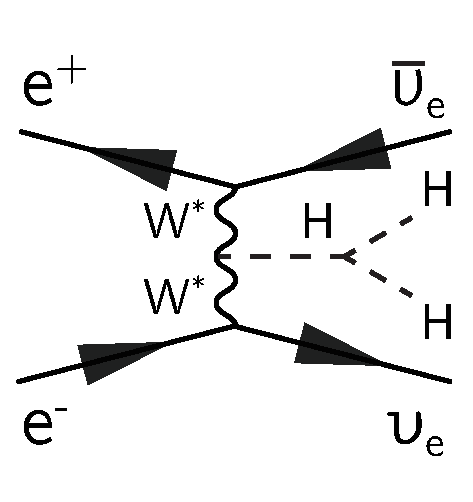
\includegraphics[width=\textwidth]{{{doubleHiggs/Feynman/1}}}
    \caption{}
    \label{fig:doubleHiggsFeynman1}
  \end{subfigure}
  \hfill
  \begin{subfigure}[b]{0.22\textwidth}
    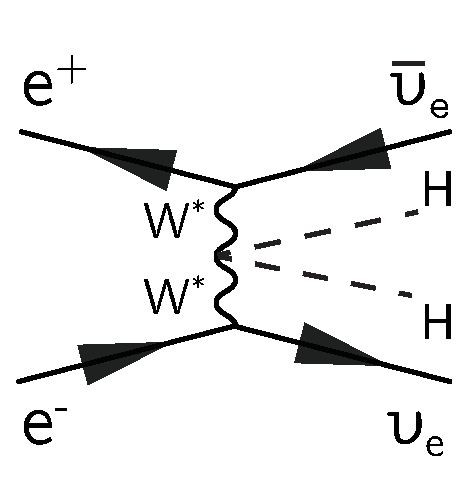
\includegraphics[width=\textwidth]{{{doubleHiggs/Feynman/2}}}
    \caption{}
    \label{fig:doubleHiggsFeynman2}
  \end{subfigure}
  \begin{subfigure}[b]{0.22\textwidth}
    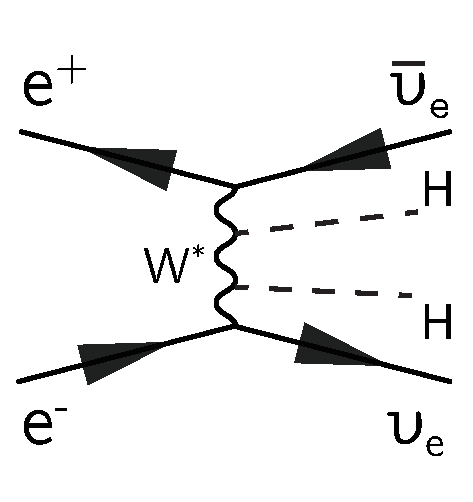
\includegraphics[width=\textwidth]{{{doubleHiggs/Feynman/3}}}
    \caption{}
    \label{fig:doubleHiggsFeynman3}
  \end{subfigure}
  \hfill
  \begin{subfigure}[b]{0.22\textwidth}
    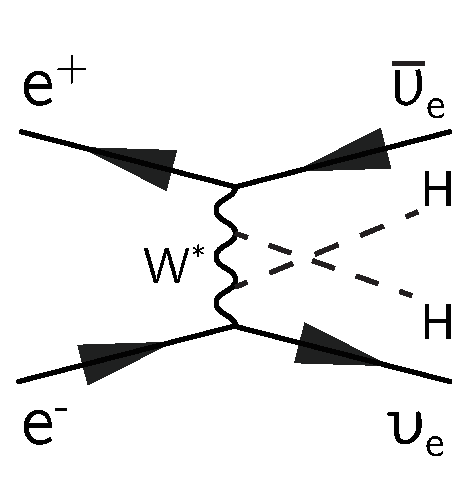
\includegraphics[width=\textwidth]{{{doubleHiggs/Feynman/4}}}
    \caption{}
    \label{fig:doubleHiggsFeynman4}
  \end{subfigure}
\caption[]%
   {Figures show Feynman diagrams of leading-order \eeToHH processes at \CLIC, without considering {\HepProcess{ \Pem \Pep \to \PZ \PHiggs \PHiggs}\xspace}. \FIGURE{fig:doubleHiggsFeynman1} is sensitive to the Higgs triple self coupling \gHHH. \FIGURE{fig:doubleHiggsFeynman2} is sensitive to quartic coupling \gWWHH.}
   \label{fig:doubleHiggsFeynman}
\end{figure}



\section{Monte Carlo Sample Generation}


% TODO
% Understand bremsstrahlung and EPA
Selected background samples are considered in the analysis and listed in Table \ref{tab:doubleHiggsMCSamples}. The signal channel is \eeToHHbbWWFull where both \PW decay hadronically. 
%The analysis is performed with \CLICILD detector concept at \rootS{1.4} and 3\,TeV, and the semi-leptonic channel. Unless specified, the

Background processes with many quarks with missing energies would be challenging to veto. Two examples  are \eeTo{ \Pquark \Pquark \Pquark \Pquark \Pnu \APnu} and \egamma{\Pem}{\Pphoton}{BS}{\Pnu \Pquark \Pquark \Pquark \Pquark}. Single Higgs boson production would be difficult to remove as well, such as \eeTo{\qlight \qlight \PHiggs \Pnu \APnu}.

Some background channels are not considered because either have different different event topologies, or they have very small cross sections. For example  \egamma{\Pepm}{\Pphoton}{}{\Pquark \Pquark \PHiggs \Plepton} is ignored as the cross section is vert small even at \rootS(3) (0.07\,fb with photon from EPA, 0.6\,fb with photon from BS). Other background channels are not simulated due to computational limitations. For example, six-quark final states were not simulated due to constraint of the simulating software.

Electron-photon interactions are considered in this analysis. They are important as the the interaction becomes significant with high \sqrtS. Processes initiated by photons included, where photons are produced due to the high electric field generated by the colliding beams. Processes invloving real photons from beamstrahlung (BS) and ``quasi-real'' photons are generated separately. For the ``quasi-real'' photon initiated processes, the Equivalent Photon Appproximation (EPA) has been used.


For processes involving Higgs production explicitly, simulated Higgs mass is 126\,GeV. Multi-quark final state background samples could, in principle, contain higgs production. Therefore, they are generated with a Higgs mass of 14\,TeV. This will produce negligible double higgs production cross section. The cross section for sub-channels of the signal, such as \eeToHHbbWW, are corrected manually according to \cite{Dittmaier:2012vm}, as the internal value of the event generation software (PYTHIA) is inaccurate.



% ATTN need to rewrite
The simulation and reconstruction chain are described in \Chapter{chap:Reconstruction}. For most background processes, events are simulated when invariant mass of quarks are above 50\,GeV. For electron-photon interaction with $\Pquark\Pquark\Pquark\Pquark\Pnu$ final state, events are simulated when invariant mass of quarks are above 120\,GeV. These limits are necessary to generate a large amount of background samples in a feasible time, without losing much signal samples.

Finally, the main beam induced background \ggHad is simulated and overlayed to all samples according to the integration time of each subdetector. Details can be found in \Section{}.

\begin{table}[!tbp]\centering
% TODO fix lumi correction for e gamma, gamma e
% TODO change some of sample cross section for  electron-photon interaction with four quarks and a neutrino final state
\small
%{

\begin{tabular}{lr}
\hline \hline
Channel  &  $\sigma(\rootS{1.4})$ / fb   \\
\hline
\eeToHH & 0.149 \\
\hline
\eeToHHbbWWFull,hadronic & 0.018  \\
\eeToHHbbbbFull & 0.047 \\
\eeToHHotherFull & 0.085 \\
\hline
\eeTo{\qlight \qlight \PHiggs \Pnu \APnu}  & 0.86 \\
\eeTo{\Pcharm \APcharm \PHiggs \Pnu \APnu}  & 0.36 \\
\eeTo{\Pbottom \APbottom \PHiggs \Pnu \APnu}  & 0.31 \\

\eeTo{ \Pquark \Pquark \Pquark \Pquark}   &   1245.1\\
\eeTo{ \Pquark \Pquark \Pquark \Pquark \Plepton \Plepton}& 62.1* \\
\eeTo{ \Pquark \Pquark \Pquark \Pquark \Plepton \Pnu}& 110.4*\\
\eeTo{ \Pquark \Pquark \Pquark \Pquark \Pnu \APnu} & 23.2* \\

\eeTo{ \Pquark \Pquark} &  4009.5\\
\eeTo{ \Pquark \Pquark \Plepton \Pnu} &  4309.7\\
\eeTo{ \Pquark \Pquark \Pl \Pl} &  2725.8 \\
\eeTo{ \Pquark \Pquark \Pnu \Pnu} & 787.7  \\
\hline
\egamma{\Pem}{\Pphoton}{BS}{\Pem \Pquark \Pquark \Pquark \Pquark} & 1160.7  \\
\egamma{\Pep}{\Pphoton}{BS}{\Pep \Pquark \Pquark \Pquark \Pquark} & 1156.3 \\
\egamma{\Pem}{\Pphoton}{EPA}{\Pem \Pquark \Pquark \Pquark \Pquark} & 287.1 \\
\egamma{\Pep}{\Pphoton}{EPA}{\Pep \Pquark \Pquark \Pquark \Pquark}  & 286.9 \\
\egamma{\Pem}{\Pphoton}{BS}{\Pnu \Pquark \Pquark \Pquark \Pquark}& 79.8\myDagger \\
\egamma{\Pep}{\Pphoton}{BS}{\APnu \Pquark \Pquark \Pquark \Pquark}& 79.3\myDagger \\
\egamma{\Pem}{\Pphoton}{EPA}{\Pnu \Pquark \Pquark \Pquark \Pquark}& 17.4\myDagger  \\
\egamma{\Pep}{\Pphoton}{EPA}{\APnu \Pquark \Pquark \Pquark \Pquark}& 17.3\myDagger  \\

\egamma{\Pem}{\Pphoton}{BS}{\Pquark \Pquark \PHiggs \Pnu} & 15.8* \\
\egamma{\Pep}{\Pphoton}{BS}{\Pquark \Pquark \PHiggs \Pnu} & 15.7* \\
\egamma{\Pem}{\Pphoton}{EPA}{\Pquark \Pquark \PHiggs \Pnu} & 3.39* \\
\egamma{\Pep}{\Pphoton}{EPA}{\Pquark \Pquark \PHiggs \Pnu} & 3.39*   \\
\hline
\gammagamma{\Pphoton}{BS}{\Pphoton}{BS}{ \Pquark \Pquark \Pquark \Pquark}& 21406.2*  \\
\gammagamma{\Pphoton}{BS}{\Pphoton}{EPA}{ \Pquark \Pquark \Pquark \Pquark}& 4018.7* \\
\gammagamma{\Pphoton}{EPA}{\Pphoton}{BS}{ \Pquark \Pquark \Pquark \Pquark}& 4034.8* \\
\gammagamma{\Pphoton}{EPA}{\Pphoton}{EPA}{ \Pquark \Pquark \Pquark \Pquark}& 753.0* \\
\hline \hline
\end{tabular}

\caption[]{List of signal and background samples with the corresponding cross sections at \rootS{1.4}. \Pquark can \Pup, \Pdown, \Pstrange, \Pbottom or \Ptop. Unless specified, \Pquark, \Plepton and \Pnu represent particles and its corresponding anti-particles. \Pphoton(BS) represents a real photon from beamstrahlung (BS). \Pphoton(EPA) represents a ``quasi-real'' photon, simulated with the Equivalent Photon Approximation. For processes involving Higgs production explicitly, simulated Higgs mass is 126\,GeV. Otherwise, Higgs mass is set to 14\,TeV. For processes labeled with * and $\myDagger$, the generator level cut requires invariant mass of quarks greater than 50 and 120\,GeV, respectively.}
\label{tab:doubleHiggsMCSamples}
\end{table}
%Simulated \PW has invariant mass of 80.385\,GeV.

\section{Physics object and event reconstruction}

The reconstruction is done via Marlin in \ilcsoft v01-16. Separate software packages (processors) exist for identification of electrons, muons, and taus, and for jet reconstruction. New processors have been developed and existing processors have been optimised for signal selection and background rejection. The latest functioning flavour tagging processor exist in \ilcsoft v01-16. Thus newer versions of  \ilcsoft can not be used in this analysis.

For the signal channel, \eeToHHbbWWHad, there is no lepton in the final state, whilst many background final states contain primary leptons, such as \HepProcess{\Pquark \Pquark \Pquark \Pquark \Plepton \Pnu}. Hence effective vetoing events with leptons would improve the signal selection efficiency. Leptons from channels like \HepProcess{\Pquark \Pquark \Pquark \Pquark \Plepton \Pnu} are primary, where their tracks are very close to the interaction point. These leptons are typically energetic, and often isolated from other particles. Whilst electrons and muons are stable enough to deposit energies in calorimeters, tau lepton is very short lived and decays in the tracker. Therefore only tau decay products can be reconstructed. These characteristics provide the basis for the isolated lepton finding.



\subsection{Electron and muon identification}
\label{sec:doubleHiggsLeptonID}


\subsubsection{IsolatedLeptonFinderProcessor}
\label{sec:doubleHiggsIsolatedLeptonFinder}
IsolatedLeptonFinderProcessor in Marlin package is used, modified, and optimised. This processor identifies high energy electrons and muons that are away from other particles, ``isolated''. The optimal parameters below are chosen in collaboration and tested using the signal channel and the \eeTo{ \Pquark \Pquark \Pquark \Pquark \Plepton \Pnu} channel.

Electrons induced electromagnetic showers are mostly contained in the \ECAL, while muons would deposit some energies in the \ECAL. The inner detector tracks of electrons and muons from the electron-positron interaction are primary tracks, which are very close to the interaction point. The isolation criteria requires the lepton to be far away from other high energy particles. These form the logics for the IsolatedLeptonFinderProcessor. The value for the selection cut is listed in \Table{tab:doubleHiggsIsolatedLeptonFinder}. $E_{\ECAL}$ is the energy deposited in the \ECAL. $E_{cone}$ is the total energy of PFOs within a cone of an opening angle of $\cos^{-1}(0.995)$ around the lepton. $d_0$, $z_0$, and $r_0$ are the Euclidean distance of the track starting point to the interaction point in the x-y plane, the in z direction, and in the x-y-z three dimensional space. The performance of the processor is shown in \Table{tab:doubleHiggsIsoLepPerformance}.


\begin{table}[!htbp]
\begin{tabular}{lr}
\hline
\hline
IsolatedLeptonFinderProcessor  & Selection \\
\hline
High Energy (GeV) &  $E > 15$  \\
Energy deposition  \Pepm & $\frac{E_{\ECAL}}{E} > 0.9$ \\
Energy deposition  \Pmupm &  $ 0.25> \frac{E_{ECAL}}{E} > 0.05$\\
Primary Track (mm) & $d_0 < 0.02, z_0 < 0.03, r_0 < 0.04$ \\
Isolation (GeV)& $E_{cone}^2 \leqslant 5.7 \times E - 50$ \\
\hline
\hline

\end{tabular}
\caption[]
{Optimised selection criterion for IsolatedLeptonFinderProcessor}
\label{tab:doubleHiggsIsolatedLeptonFinder}
\end{table}

\subsubsection{BonoLeptonFinderProcessor}
\label{sec:doubleHiggsBonoLeptonFinder}
The analysis would benefit from aggressive lepton veto due to the low signal cross section. Since the IsolatedLeptonFinderProcessor is conservative, an aggressive light lepton selection processor, BonoLeptonFinderProcessor, is developed. It utilises calorimetric information provided by \pandora.

The processor uses two sets of cuts and the logic is similar to ones in the IsolatedLeptonFinderProcessor. The first set of cuts uses the particle ID information from \pandora. The cuts require a \pandora electron or muon with high \pT and is from a primary track. The lepton should either have very high transverse momentum, or it is isolated. The second set of cuts uses \ECAL energy fraction to determine light leptons. The rest of the logic is very similar to the first set. The isolation criterion is stricter than it in the first set to reduce fake rate.

\begin{table}[!htbp]
\begin{tabular}{lr}
\hline
\hline
BonoLeptonFinderProcessor  & Selection \\
\hline
High Energy (GeV) &  $E > 10$  \\
Energy deposition  \Pepm & \pandora reconstructed \& $\frac{E_{\ECAL}}{E} > 0.95$ \\
Energy deposition  \Pmupm &  \pandora reconstructed\\
Primary Track (mm) & $r_0 < 0.015$ \\
a) High Transverse Momentum (GeV) &  $\pT > 40$  \\
b) Isolation (GeV)& $E \geqslant 23 \times \sqrt{E_{cone1}} + 5$ \\
\hline
High Energy (GeV) &  $E > 10$  \\
Energy deposition  \Pepm & $\frac{E_{\ECAL}}{E} > 0.95$ \\
Energy deposition  \Pmupm & $0.2 > \frac{E_{\ECAL}}{E} > 0.05$ \\
Primary Track (mm) & $r_0 < 0.5$ \\
a) High Transverse Momentum (GeV) &  $\pT > 40$  \\
b) Isolation (GeV)& $ E \geqslant 28 \times \sqrt{E_{cone2}} + 30$ \\
\hline
\hline

\end{tabular}
\caption[]
{Optimised selection criterion for IsolatedLeptonFinderProcessor}
\label{tab:doubleHiggsBonoLeptonFinder}
\end{table}

\TABLE{tab:doubleHiggsBonoLeptonFinder} lists  values for the selection cut. Variables are defined similarly as those in \Section{sec:doubleHiggsIsolatedLeptonFinder}. \pT is the transverse momentum. $E_{cone1}$ and $E_{cone2}$ are the total energy of PFOs within a cone of an opening angle of $\cos^{-1}(0.995)$ and $\cos^{-1}(0.99)$ respectively around the lepton. The performance of the processor is shown in \Table{tab:doubleHiggsIsoLepPerformance}.


\subsubsection{Comparison: IsolatedLeptonFinderProcessor v.s. BonoLeptonFinderProcessor}


Two processors share similar criterion for light lepton identification. The main difference is that the BonoLeptonFinderProcessor uses the particle identification from \pandora, use extra calorimetric information to determine the particle ID than simple \ECAL energy fraction. BonoLeptonFinderProcessor also allows high \pT light lepton to be identified in a potential non-isolated environment, which leads to the more aggressive nature of the BonoLeptonFinderProcessor. The performance of two processors on the signal and selected background samples is shown in \Table{tab:doubleHiggsIsoLepPerformance}.

\subsection{Tau identification}

\subsubsection{TauFinderProcessor}

% TODO check tau stuff
With a decay length of 87$\mu{m}$, tau leptons decay before reaching the detector and can only be identified through the reconstruction of their decay products. The leptonic decay of tau can be identified using the two isolated lepton finder processors in \Section{sec:doubleHiggsIsolatedLeptonFinder} and  \Section{sec:doubleHiggsBonoLeptonFinder}. Therefore tau identification will focus on the hadronic decay.

The basic logic of a tau finder is similar to a cone clustering algorithm (\Section{sec:pandoraConeCluster}). A high energy track is selected as a seed and a small cone is formed around it. The PFOs inside the cone are required to be consistent with a tau hadronic decay: no more than 3 charged particles, invariant mass close to tau mass and few PFOs in the cone. The cone then forms the tau candidate. Like the lepton in the isolated light lepton finder, the tau candidate is required to be isolated from other particles. To reduce fake rate, low momentum and very forward particles do not participate in the tau finding, as they more likely come from \ggHad background.

TauFinderProcessor \cite{LCD-Note-2010-009}, an existing processor Marlin package, has been tuned in collaboration and tested. The selection criterion are listed in \Table{tab:doubleHiggsTauFinderProcessor}. Variables are defined similarly as those in previous sections. $\theta_Z$ is the polar angle w.r.t. the beam axis. $N_{X^+} > 3$ and $N_{cone}$ are number of charged particles and number of PFOs respectively in the tau candidate. $m_{cone}$ is the invariant mass of the sum of the PFOs, tau candidate. $E_{cone}$ are the total energy of PFOs within a cone of an opening angle between 0.03 and 0.33\,rad  around the tau seed. The performance of the processor is shown in \Table{tab:doubleHiggsIsoLepPerformance}.

\begin{table}[!htbp]
\begin{tabular}{lr}
\hline
\hline
TauFinderProcessor  & Selection \\
\hline
Veto \ggHad (GeV) &  $\pT < 1$, $\absOf{\cos\left(\theta_Z\right)} > 1.1$  \\
Seed particle (GeV) & $\pT > 10$ \\
Tau candidate cone opening angle (rad) & 0.03 \\
Tau candidate rejection & $N_{X^+} > 3$, $N_{cone} > 10$, $m_{cone} > 2$   \\
Isolation (GeV)&  $ E_{cone} < 3$\\
\hline
\hline

\end{tabular}
\caption[]
{Optimised selection criterion for TauFinderProcessor}
\label{tab:doubleHiggsTauFinderProcessor}
\end{table}

\subsubsection{BonoTauFinderProcessor}

For the similar reason of developing a more agressive light lepton finder, a new more aggressive tau lepton selection processor, BonoTauFinderProcessor, is developed.  BonoTauFinderProcessor utilises calorimetric information provided by PandoraPFA and has a cleaner code structure.

Similar to TauFinderProcessor, this processor identifies a high momentum particle as a tau seed. Particles are iteratively added to the search cone according to the size of the opening angle to the seed. After each particle addition, a temporary search cone is cone is then considered as the tau candidate, and tested against tau hadronic decay hypothesis and isolation conditions. The tau candidate only needs to pass one of the isolation conditions. The iterative particle addition would stop when the cone opening angle is bigger than a threshold. If multiple temporary search cones of a same seed passing the selection, the cone with smallest opening angle is chosen to form the final tau candidate. To reduce fake tau decay products from from \ggHad background, low energy particles do not participate in the tau finding.

\TABLE{tab:doubleHiggsTauFinderProcessor} lists the selection criterion for BonoTauFinderProcessor. Variables are defined similarly as those in previous sections. $\theta_S$ is the opening angle of the search cone. $cone1$ and $cone2$ are defined as a cone of an opening angle of $\cos^{-1}(0.95)$, and $\cos^{-1}(0.99)$ respectively around the tau seed. $r_0$ is referring to tau seed particle. The performance of the processor is shown in \Table{tab:doubleHiggsIsoLepPerformance}.



\begin{table}[!htbp]
\begin{tabular}{lr}
\hline
\hline
TauFinderProcessor  & Selection \\
\hline
Veto \ggHad (GeV) &  $E < 1$\\
Seed particle (GeV) & $\pT > 5$ \\
Maximum search cone opening angle (rad) & $\theta_S \leqslant \cos^{-1}(0.999)$\\
Tau candidate rejection & $N_{X^+} \neq 1,3$, $m_{PFO} > 3$   \\
Isolation (GeV) 1& $N_{cone1} = 0$, $ \pT_{cone} \geqslant 10$\\
Isolation (GeV) 2& $N_{X^+} = 1$, $N_{cone1} = 1$, $r_0 > 0.01$\\
Isolation (GeV) 3& \multicolumn{1}{R{0.4\textwidth}}{{$N_{X^+} = 3$, $N_{cone1} = 1$, $ \pT_{cone} \geqslant 10$, $\theta_S < \cos^{-1}(0.9995)$}}\\
Isolation (GeV) 4& \multicolumn{1}{R{0.4\textwidth}}{$N_{X^+} = 1$, $N_{cone2} = 0$, $r_0 > 0.01$, $ \pT_{cone} \geqslant 10$}\\
Isolation (GeV) 5& \multicolumn{1}{R{0.4\textwidth}}{{$N_{X^+} = 3$, $N_{cone2} = 0$, $ \pT_{cone} \geqslant 10$, $\theta_S < \cos^{-1}(0.9995)$}}\\
\hline
\hline

\end{tabular}
\caption[]
{Optimised selection criterion for BonoTauFinderProcessor}
\label{tab:doubleHiggsBonoTauFinderProcessor}
\end{table}


\subsubsection{Comparison: TauFinderProcessor v.s. BonoTauFinderProcessor}

Two processors share similar size of search cone and isolation cone.  The main difference is that the BonoTauFinderProcessor has an interactive approach to build up tau candidate, which allows a dynamic tau search cone size. The BonoTauFinderProcessor has looser cut on minimum \pT and invariant, but stricter isolation criterion. This leads to a more aggressive tau finder. The performance of processors is shown in \Table{tab:doubleHiggsIsoLepPerformance}.

\subsection{Very forward electron identification}

At high \sqrtS, particles are boosted and it is important to extract information in the forward calorimeters to aid signal selection. Certain background channels, for example photon-electron interactions, can have energetic electrons in  the forward calorimeters, the \LumiCAL and the \BeamCAL. These extracting information from these forward calorimeters is different to information in the barrel and the end cap. As forward calorimeters have the angular low angular acceptance, most particles in these forward detector would be very forward particles from beam induced background. However, previous study \cite{sailer2012radiation} has shown that sufficiently high energy electrons can be efficiently identified in the \BeamCAL and \LumiCAl. 

For the \CLICILD detector concept, energies deposited in the \LumiCAL and the \BeamCAL are not simulated. This is because the thousands of beam induced background particles per bunch corssing () (see \Section{}) requires expensive computational resources. The current simulation software could not handle the simulation in a feasible time. Therefore, the adopted approach is to parameterise the background particle energy deposition and leads to electron tagging algorithms.

For the \BeamCAL, \cite{Sailer:2017onh} describes an electron tagging algorithm developed using \rootS{3} collision environment, by comparing the simulated electron and background energy distributions. An electron is tagged if the energy is significantly larger than the expected background energy distributions.

Events are overlaid with background energy deposition integrated over 40 bunch crossing. A C++ code library has been developed and used in this analysis. The tagging efficiency for electrons with energy 500 to 1500\,GeV are bin in histograms at interval of 100\,GeV. There is no tagging for electrons with energy below 500\,GeV or about 1500\,GeV. An indicative performance plot of 500\,GeV electron tagging efficiency as a function of the polar angle is shown in \Figure{fig:doubleHiggsForwardBCAL}.


The input of the \BeamCAL electron tagging algorithm is the four momenta of the MC electron. Since the algorithm assumes collision at \rootS{3}, for the \rootS{1.4} user case, the momenta of the MC electron is scaled down by a factor of $\frac{3}{1.4}$ to use the algorithm.
\begin{figure}[!tbp]
  \begin{subfigure}[b]{0.45\textwidth}
    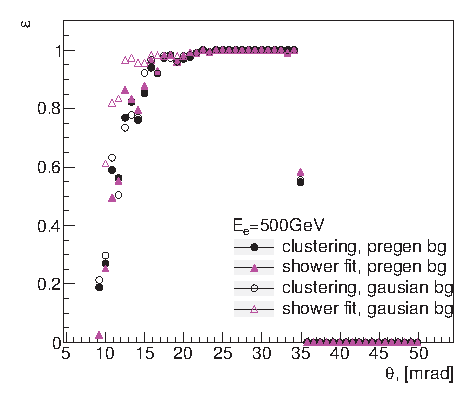
\includegraphics[width=\textwidth]{{{doubleHiggs/forward/ForwardBCAL}}}
    \caption{}
    \label{fig:doubleHiggsForwardBCAL}
  \end{subfigure}
  \hfill
  \begin{subfigure}[b]{0.45\textwidth}
    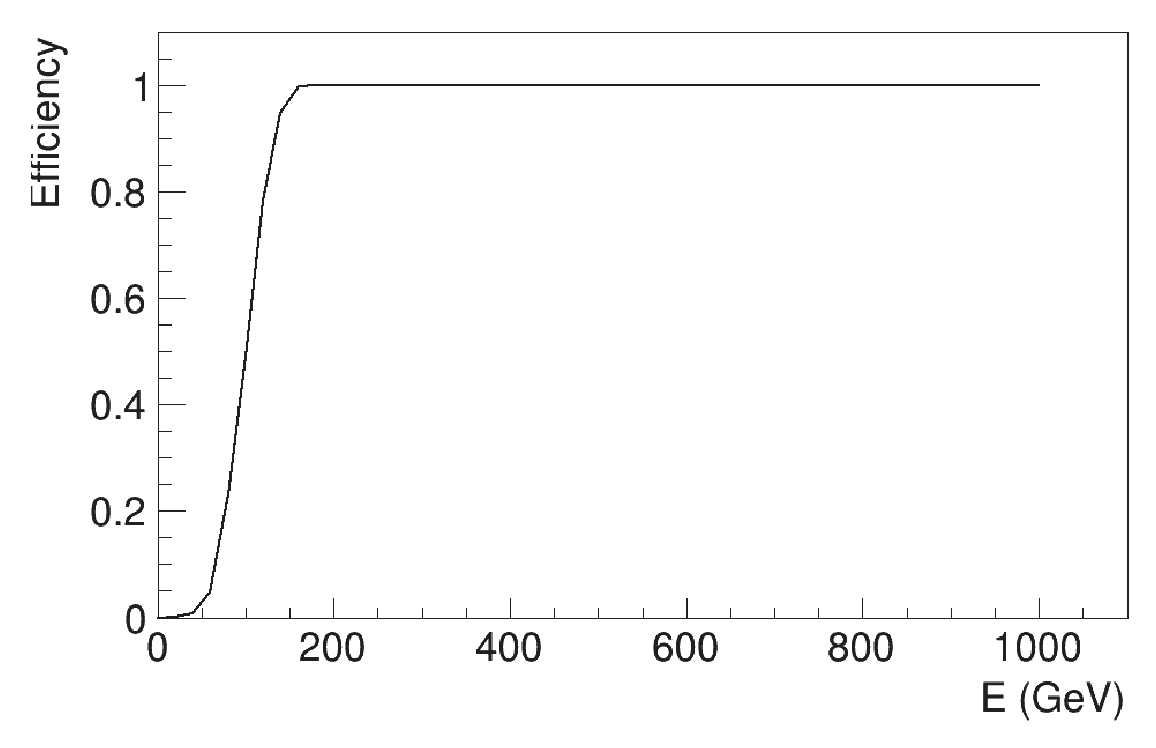
\includegraphics[width=\textwidth]{{{doubleHiggs/forward/ForwardLCAL}}}
    \caption{}
    \label{fig:doubleHiggsForwardLCAL}
  \end{subfigure}
\caption[]%
   {\FIGURE{fig:doubleHiggsForwardBCAL} shows \BeamCAL 500\,GeV electron tagging efficiency as a function of the polar angle with different methods to model backgrounds and fittings, taken from \cite{Sailer:2017onh}. \FIGURE{fig:doubleHiggsForwardLCAL} shows the \LumiCAL  electron tagging efficiency as a function of the electron energy, for polar angle $\theta = 50\,mrad$, taken from \cite{Lukic:forwardElectron}. }
   \label{fig:doubleHiggsForwardCAL}
\end{figure}

For the \LumiCAL, the \HepProcess{\PHiggs \to \Pmu \Pmu} analysis in \cite{Milutinovic-Dumbelovic:2014uta,Grefe:2012rt} has developed an algorithm for electron tagging in the \LumiCAL, with similar logic as the algorithm for the \BeamCAL. \FIGURE{fig:doubleHiggsForwardCAL} shows the \LumiCAL  electron tagging efficiency as a function of the electron energy, for polar angle $\theta = 50\,mrad$, where events are overlaid with background energy deposition integrated over 100 bunch crossings. As it is the only available performance plot for the \LumiCAL electron tagging, the electron tagging in the \LumiCAL in this analysis is based on the efficiency plot  \Figure{fig:doubleHiggsForwardCAL}.

Assuming the \LumiCAL electron tagging efficiency is described as in \Figure{fig:doubleHiggsForwardCAL}, for all polar angles and for \rootS{1.4} and 3\,TeV, \LumiCAL electrons tagging efficiency, $\varepsilon$, is parameterised as 
\begin{equation}
\varepsilon=
\begin{cases}
  0, & \text{if}\ E < 50\,GeV\\
  0.99 \times \frac{(erf(E - 100) + 1 )}{2}, & \text{otherwise}
\end{cases}
\end{equation}
where $E$ is the energy of the electron or the photon. $erf$ is the error function. For each MC electron in the \LumiCAL, a random number between 0 and 1 is generated. If the random number is less than \varepsilon, then the MC electron is tagged.

Due to lack of tracking ability in the forward region (see \Section{} and \Section{} for detector coverage), electrons and photons would have the same electromagnetic shower profile (see \Section{}), with the \ECAL spatial resolution. Therefore, MC photons and electrons appear indistinguishable to the \BeamCAL and \LumiCAL and both  are tagged by the above algorithms.


 %Due to the lack of tracking in these region, electrons and photons would have the same electromagnetic shower profile, with the given calorimeter resolution. MC photons and electrons are checked if they fall in the LCal or the BCal, and checked against the known detection efficiency.


%With the increase of the centre-of-mass energy, more  As discussed before, veto events with leptons help the signal selection. Hence the goal is to identify leptons in the forward region.

%These forward calorimeters were not simulated due to computational limitation.
% For \rootS(3), the BeamCal detection efficiency is provided by a software package \cite{}. For \rootS(1.4), the same software for the BeamCal is used, by scaling the energy of the MC particle by a factor of $\frac{3}{1.4}$. For the LumiCal, the identification efficiency is defined as


\subsection{Lepton identification performance}

The performance of two processors on the signal and selected background samples is shown in \Table{tab:doubleHiggsIsoLepPerformance}. The number is the fraction of events without identified lepton from individual processor, and combined. For both centre-of-mass, the developed version of lepton finding processors, BonoLeptonFinderProcessor and BonoTauFinderProcessor are more aggressive at rejecting background than the processors in Marlin, IsolatedLeptonFinderProcessor and TauFinderProcessor.

\begin{table}[!tbp]
\begin{tabular}{lrr}
\hline
\hline
Efficiency (1.4\,TeV)  &  Signal & \HepProcess{\Pep \Pem \to \Pquark\Pquark\Pquark\Pquark\Plepton\Pnu} \\
\hline
IsolatedLeptonFinderProcessor & 99.3\% & 50.3\%  \\
BonoLeptonFinderProcessor & 99.1\% & 39.9\%  \\
TauFinderProcessor & 97.5\% & 52.3\%  \\
BonoTauFinderProcessor & 89.7\% & 38.5\%  \\
ForwardFinderProcessor & 98.9\% & 95.1\%  \\
Combined & 86.6\% & 16.8\%  \\
\hline
\hline

\end{tabular}
\caption{isolated lepton finder processors performance on the signal and selected background samples.}
\label{tab:doubleHiggsIsoLepPerformance}
\end{table}



The background rejection is significant, shown in \Table{} for the signal and selected background.


\begin{table}[!tbp]
\begin{tabular}{lrr}
\hline
\hline
Selection / Efficiency (1.4\,TeV)  &  Signal & \egamma{\Pem}{\Pphoton}{BS}{\Pem \Pquark \Pquark \Pquark \Pquark}  \\
\hline
Combined light lepton finder & 87.6\% & 67.5\%  \\
ForwardFinderProcessor & 98.9\% & 53.6\%  \\
Combined & 86.6\% & 30.8\%  \\
\hline
\hline

\end{tabular}
\caption{Very forward electron and photon finder performance on the signal and selected background samples.}
\label{tab:doubleHiggsForwardPerformance}
\end{table}

\subsection{Other lepton identification processors}

Other isolated lepton selection processors available in Marlin package, including IsolatedLeptonTagging and TauJetClustering, have been tested. The results, after some tuning of parameters, were unsatisfactory. They either performed poorly comparing to the processors above, or became redundant after the processors above. Therefore, these processors were not used in this analysis.




\section{Jet reconstruction}

The signal channel, \eeToHHbbWWHad, is a four-jet final state. A useful technique for the analysis is to reconstruct the four-jet final state using jet algorithms. This allows discriminative variables to be calculated.

\subsection{Jet reconstruction optimisation}
\label{sec:doubleHiggsJetOptimisation}
Longitudinal invariant, \kt, jet algorithm was chosen for the jet clustering. Due to the presence high level of beam induced background at the CLIC, it has been shown that a jet algorithm designed for hadron colliders are more effective than those traditional designed for the electron-positron collider, such as Durham algorithm.\cite{}

% ATTN, PFO collection should be explained already
The free parameters for \kt algorithm is the $R$ parameter, which controls the fatness of the jet. There is also the choice of the PFO collection, which incorporate different level of time and \pT cuts, to reduce beam induce background. Both parameters are optimised for \rootS{1.4} and \rootS{3}.

The details of jet algorithm can be found in \Section{}.

The $R$ parameter of the \kt jet algorithm, and the collection of the PFOs are chosen to give the best invariant mass resolution. When there are a few suitable candidate, analysis were performed in parallel. Decision were made to give the highest signal significance.

\kt jet algorithm was used as part of the FastJet algorithms available in the Marlin package.

The samples containing the signal, \eeToHHbbWWHad, was used for the optimisation of the jet reconstruction. The signal events were chosen using MC truth information.

Jet algorithm was run in exclusive mode, where number of jets is chosen to be six.

For the signal, \eeToHHbbWWHad, one Higgs decays to two \Pbottom quarks, resulting in two jets from hadronisation. Similarly the other Higgs decays to two \PW bosons, where each \PW boson decays into two quarks. Therefore, the expected number of jets is six.

Jets produced by the \kt jet algorithm are pairred up using MC truth information, to the corresponding Higgs and \PW boson. Four invariant mass distributions are obtained: two Higgs masses, $m_{\Hbb}$, $m_{\HWW}$, and two \PW masses $m_{\PW}$, $m_{\W*}$. \W* indicates the off-mass-shell \PW boson, because when a Higgs decays into two \PW bosons, one \PW is off the mass shell, as the Higgs mass is less than the sum two \PW masses.



Three mass distributions are worth comparing for different jet reconstruction, namely, $m_{\Hbb}$, $m_{\HWW}$, and $m_{\PW}$. The ideal jet reconstruction should produce the a sharp mass peak around the particle's true mass.

To quantitatively access the mass distribution, a gaussian like fit is performed to extract the position of the peak, and the width of the distribution. The fit has the form:

\begin{equation}
f(m)=A e^{- \frac{(m - \mu)^2}{g}}
\begin{cases}
  g = 2\sigma_L + \alpha_L(m - \mu), & \text{if}\ m < \mu\\
  g = 2\sigma_R + \alpha_R(m - \mu), & \text{if}\ m \geqslant \mu
\end{cases}
\end{equation}
The fit represents an asymmetrical gaussian function, where $m$ is binned mass distribution, with 50 bins in range [0, 200]\,GeV. The fitted mass peak is denoted by $\mu$. $\sigma_L$ and $\sigma_R$ allow asymmetrical width of the distribution. $\alpha$ parameter controls the fit of tails. Inspired by the $\Ptop\APtop$  analysis \cite{}, the use of the $\alpha$ parameter allows the fit in the whole mass range, otherwise only the peak of the distribution should be fitted with a gaussian like function. $A$ is the normalistion factor. An example of the fit of $m_{\Hbb}$ is shown in \Figure{fig:doubleHiggsFitMCMass}.

\begin{figure}[!tbp]
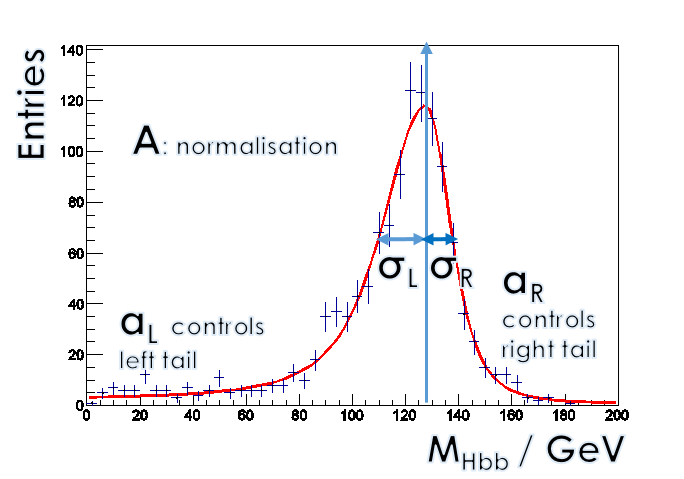
\includegraphics[width=\largefigwidth]{doubleHiggs/MCmassFit}
\caption[Example MC mass fit for double higgs analysis]%
   {A typical example of MC mass fit of $m_{\Hbb}$ for double higgs analysis. Red line indicates the best fit. Vertical arrow indicates the fitted peak position.}
   \label{fig:doubleHiggsFitMCMass}
\end{figure}

For \rootS{1.4}, shown in \Figure{fig:doubleHiggs1.4TeVMassFit}, \normalPFO with $R = 0.7$ give a good fitted mass for \HWW and \PW. The mass is slightly too low for the \Hbb. \Figure{fig:doubleHiggs1.4TeVSigmaFit} shows the combined relative fitted width for the \Hbb, \HWW and \PW. \NormalPFO with $R = 0.7$ gives an almost optimal relative width for \Hbb, while achieving a good balance for \HWW and \PW. Therefore, \normalPFO with $R = 0.7$ is chosen to be the optimal jet reconstruction parameters.

\begin{figure}[!tbp]
  \begin{subfigure}[b]{0.45\textwidth}
    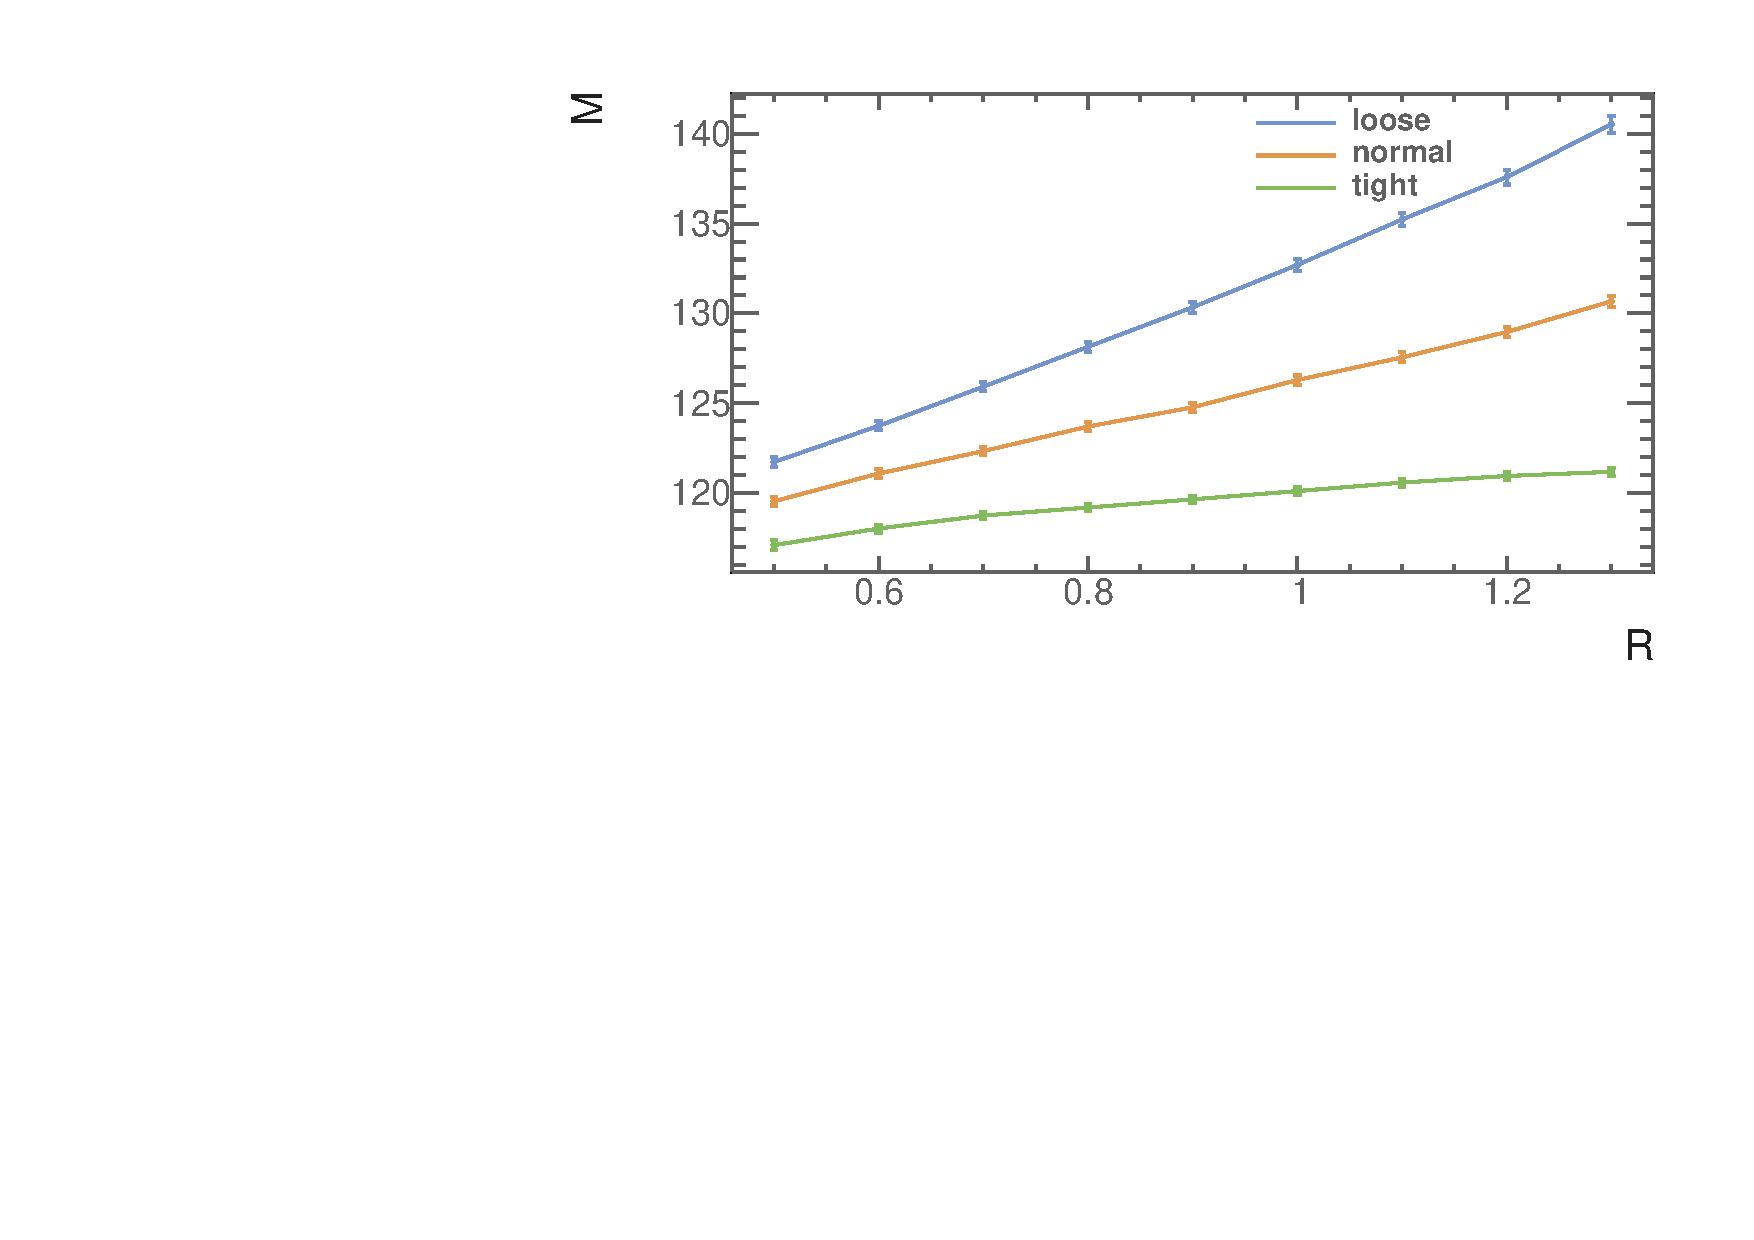
\includegraphics[width=\textwidth]{{{doubleHiggs/resolution/ILD_1.4TeV_Higgs1_M_R}}}
    \caption{}
    \label{fig:doubleHiggs1.4Higgs1M}
  \end{subfigure}
  \hfill
  \begin{subfigure}[b]{0.45\textwidth}
    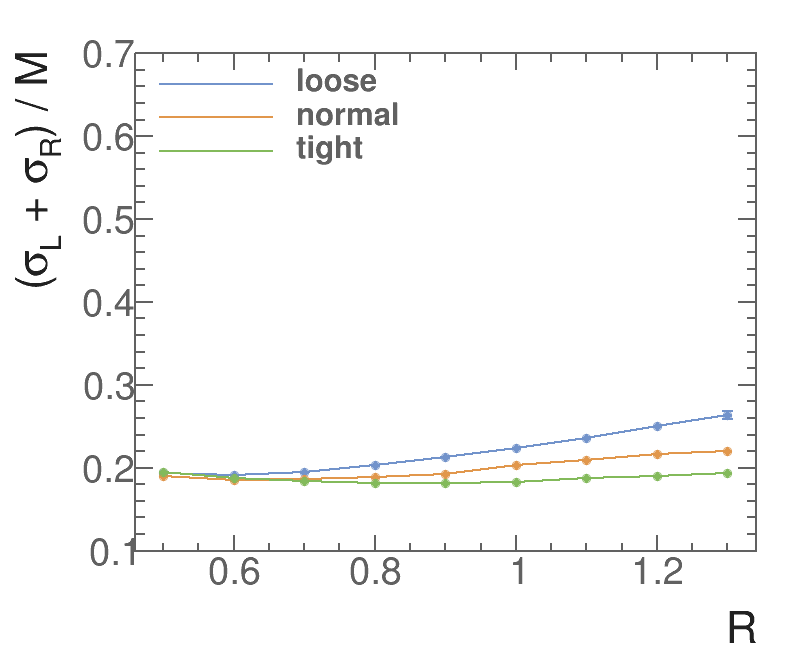
\includegraphics[width=\textwidth]{{{doubleHiggs/resolution/ILD_1.4TeV_Higgs1_SigmaL_add_SigmaR_divide_M_testR}}}
    \caption{}
    \label{fig:doubleHiggs1.4Higgs1Sigma}
  \end{subfigure}

  \begin{subfigure}[b]{0.45\textwidth}
    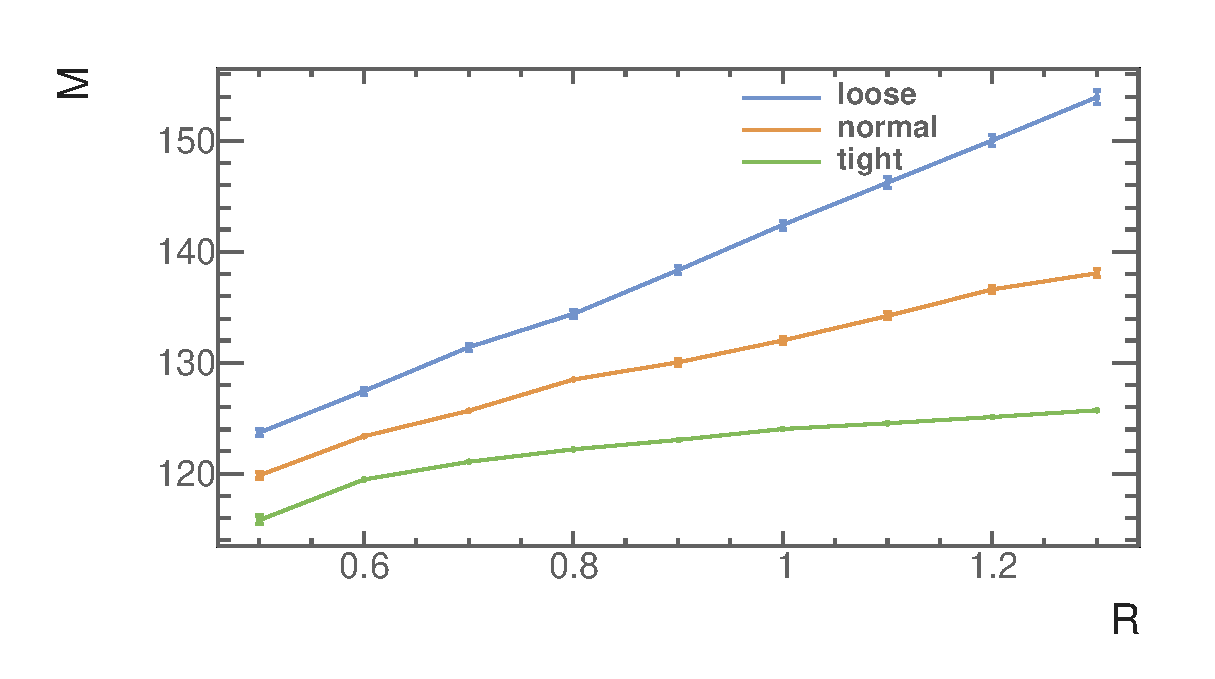
\includegraphics[width=\textwidth]{{{doubleHiggs/resolution/ILD_1.4TeV_Higgs2_M_R}}}
    \caption{}
    \label{fig:doubleHiggs1.4Higgs2M}
  \end{subfigure}
  \hfill
  \begin{subfigure}[b]{0.45\textwidth}
    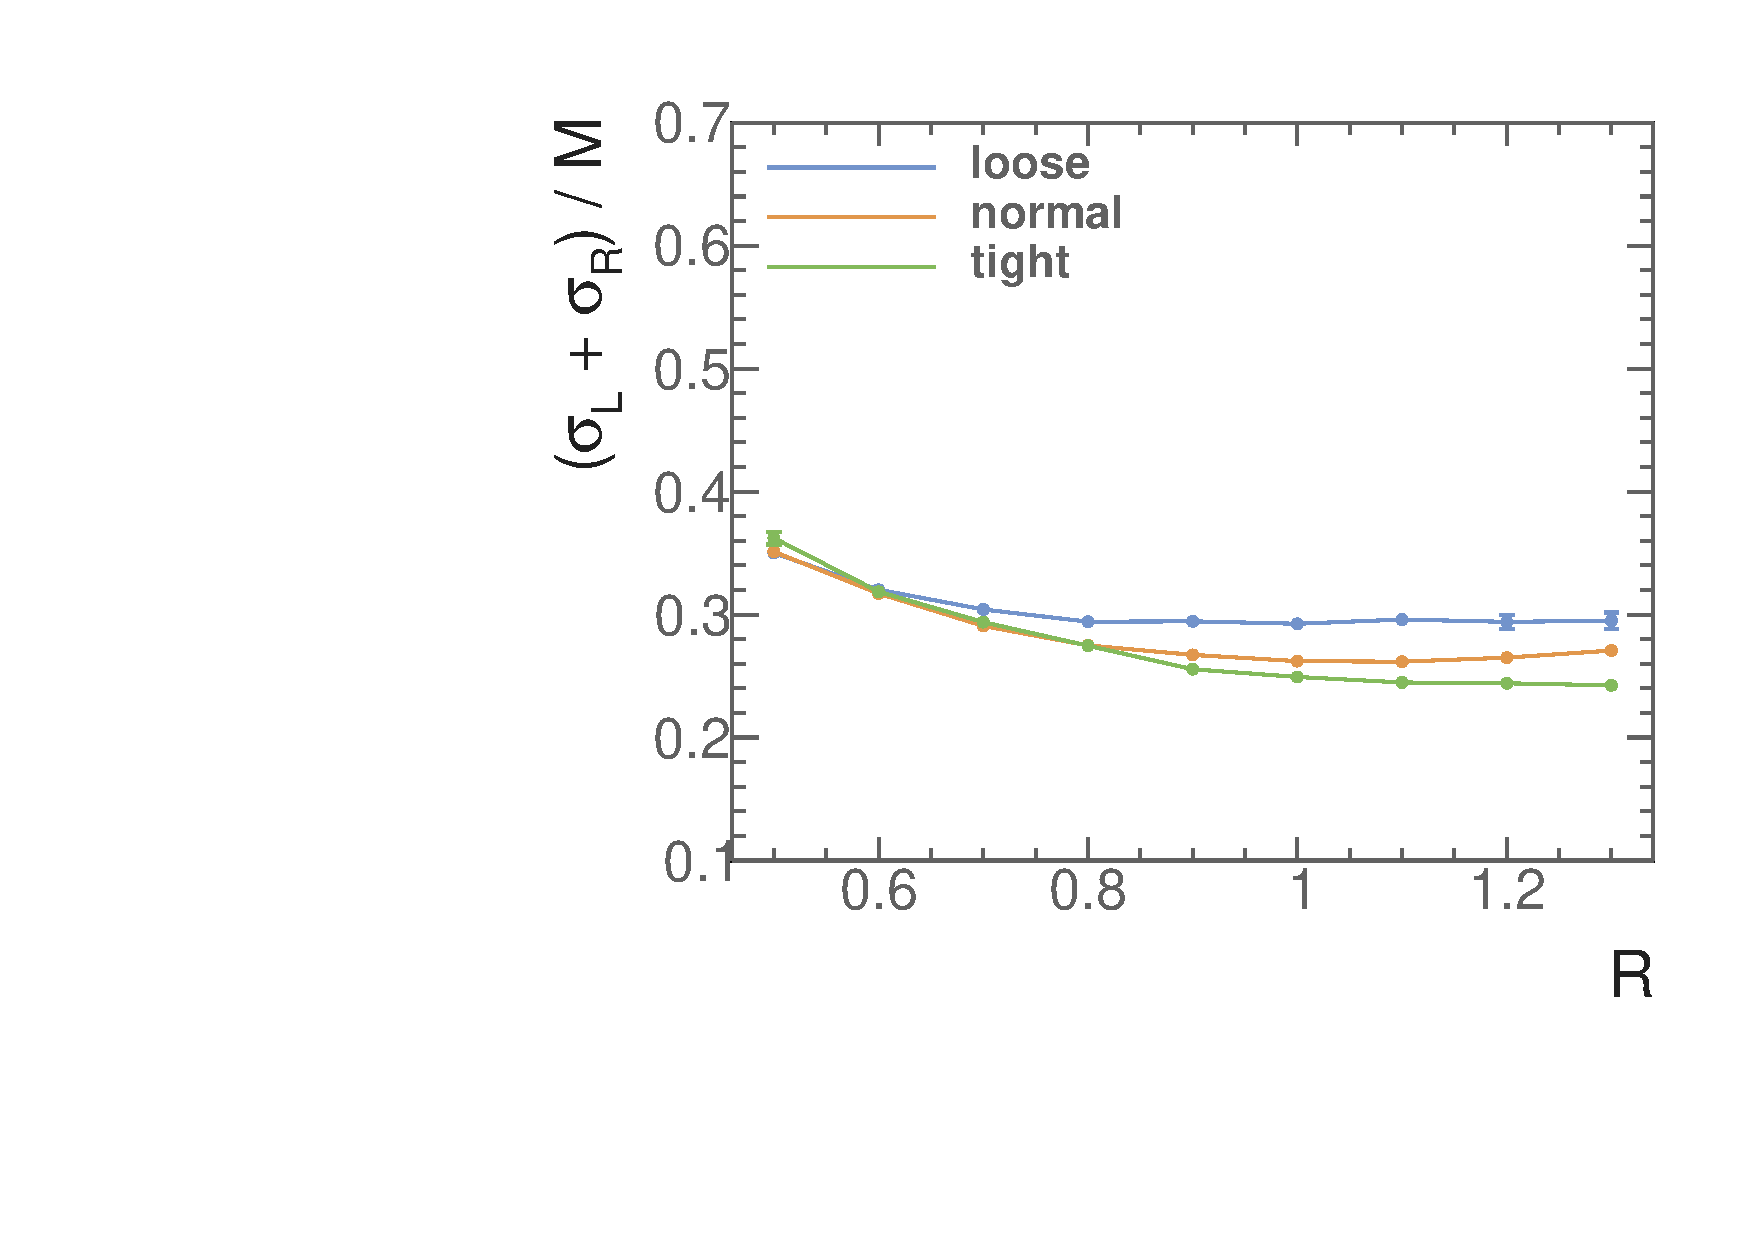
\includegraphics[width=\textwidth]{{{doubleHiggs/resolution/ILD_1.4TeV_Higgs2_SigmaL_add_SigmaR_divide_M_testR}}}
    \caption{}
    \label{fig:doubleHiggs1.4Higgs2Sigma}
  \end{subfigure}

  \begin{subfigure}[b]{0.45\textwidth}
    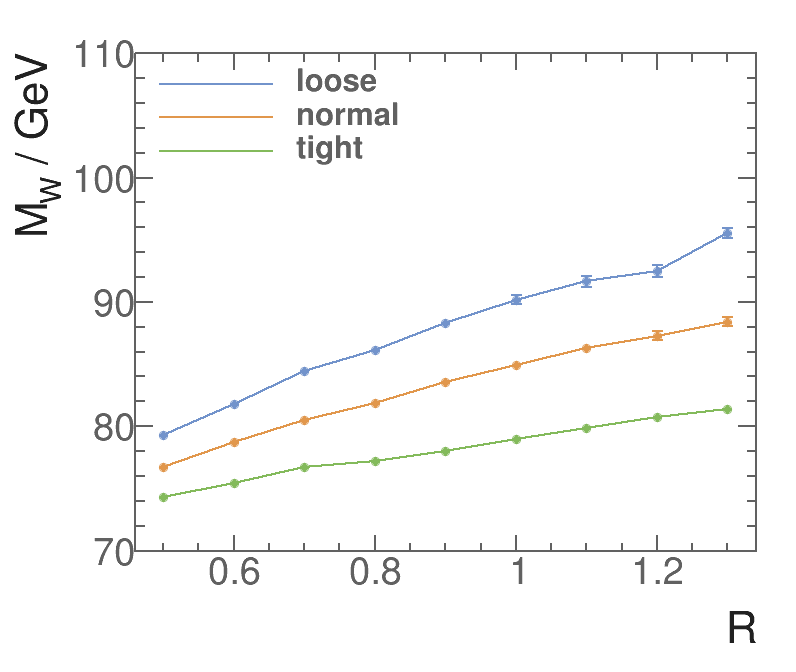
\includegraphics[width=\textwidth]{{{doubleHiggs/resolution/ILD_1.4TeV_W_M_testR}}}
    \caption{}
    \label{fig:doubleHiggs1.4WM}
  \end{subfigure}
  \hfill
  \begin{subfigure}[b]{0.45\textwidth}
    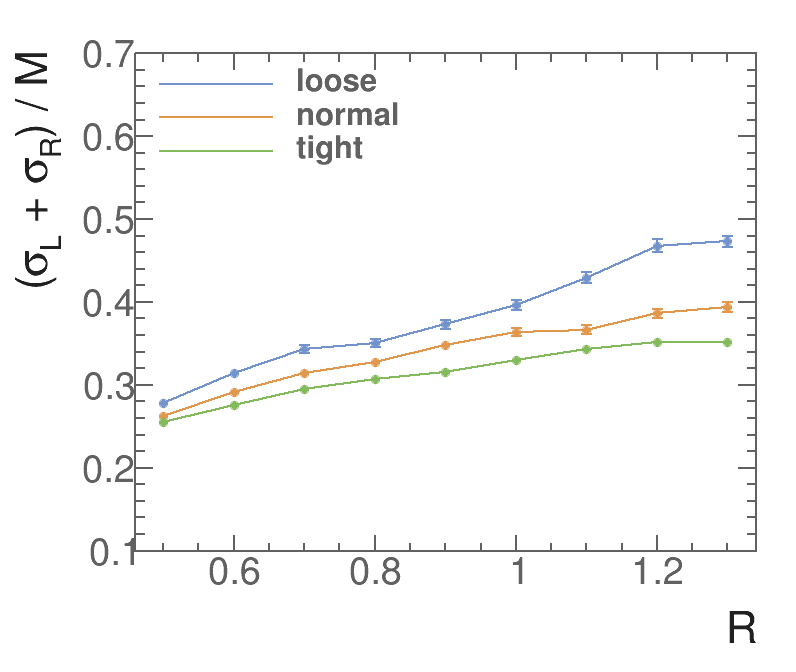
\includegraphics[width=\textwidth]{{{doubleHiggs/resolution/ILD_1.4TeV_W_SigmaL_add_SigmaR_divide_M_testR}}}
    \caption{}
    \label{fig:doubleHiggs1.4WSigma}
  \end{subfigure}

%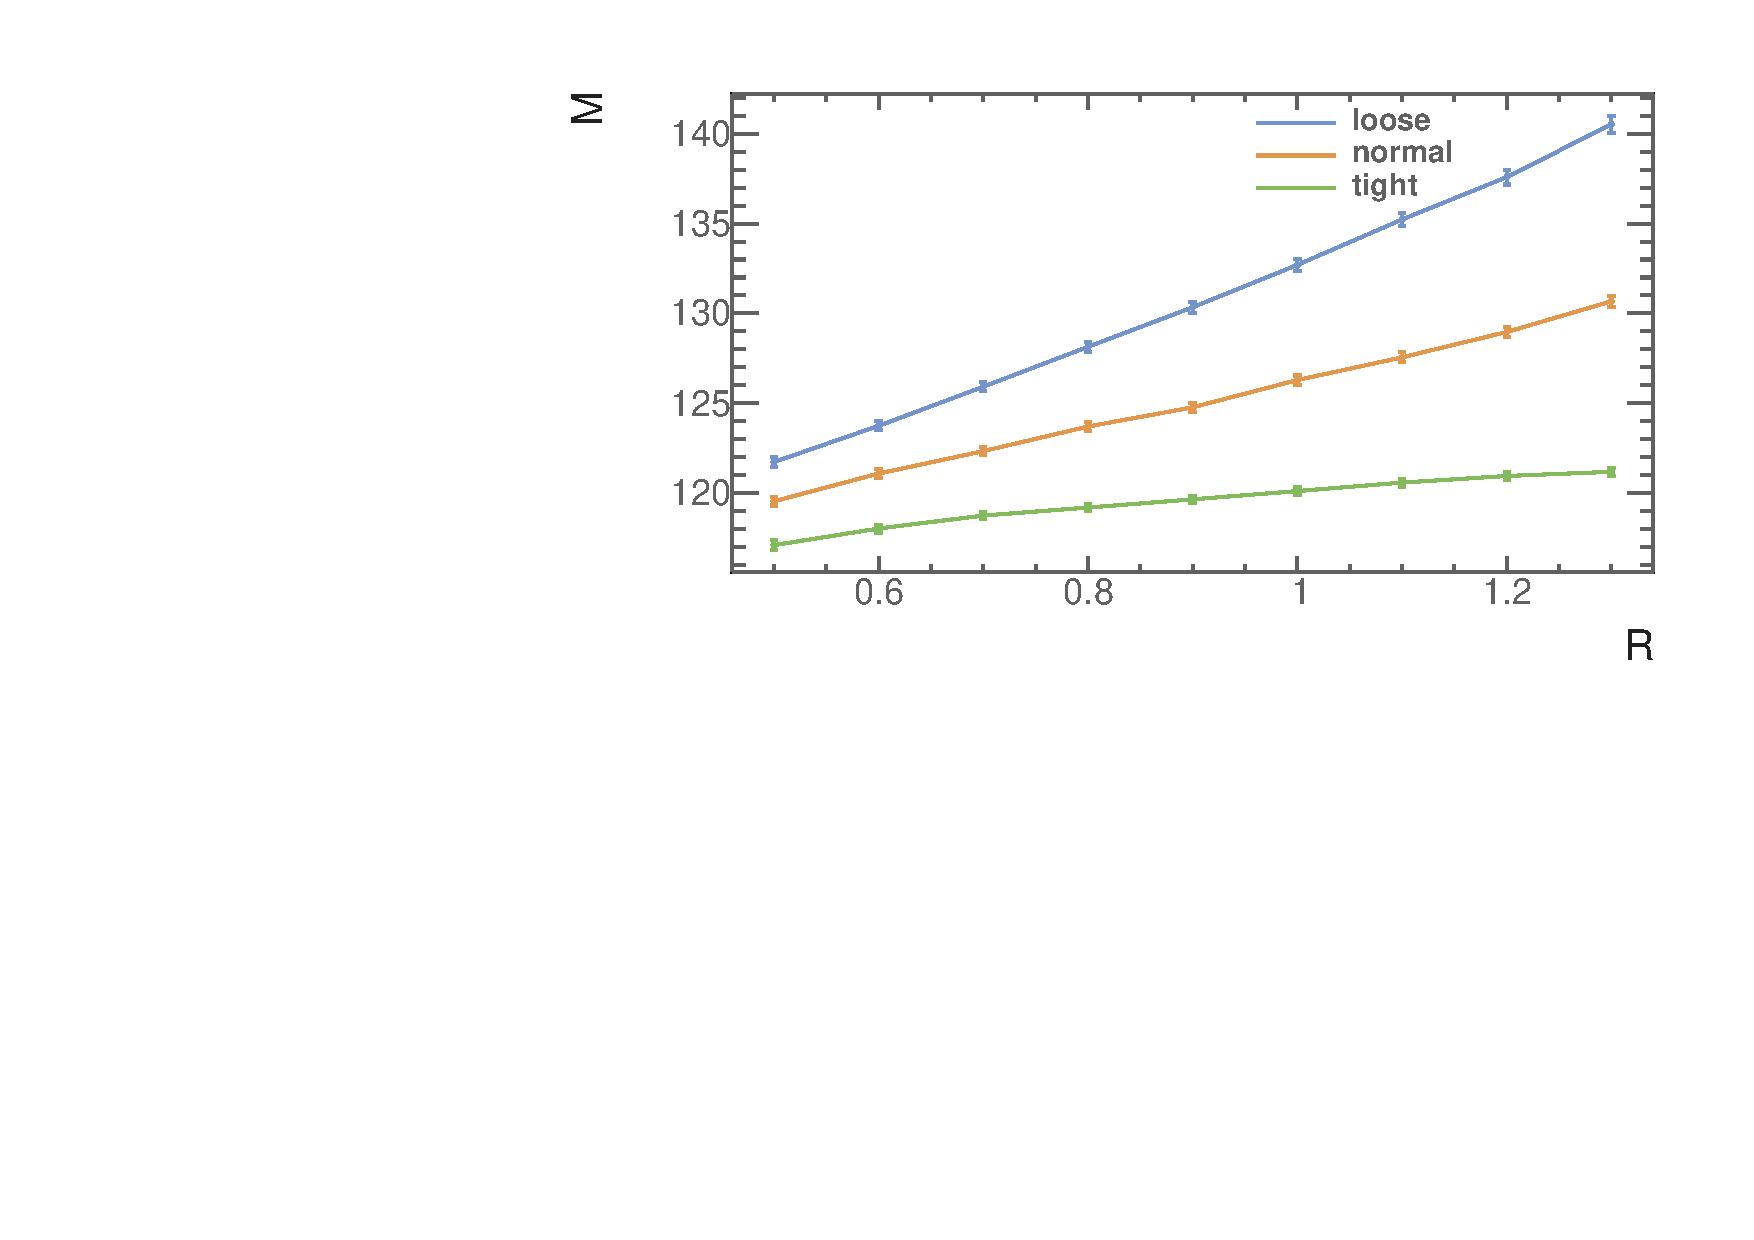
\includegraphics[width=\largefigwidth]{{{doubleHiggs/resolution/ILD_1.4TeV_Higgs1_M_R}}} \\
%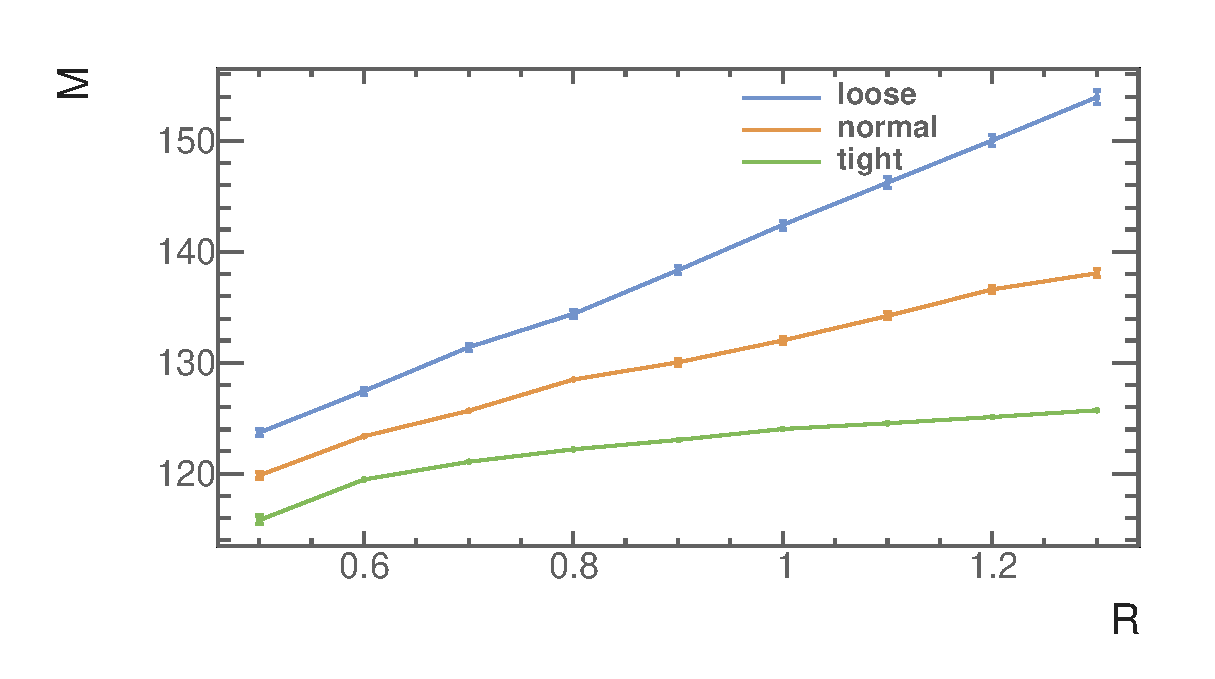
\includegraphics[width=\largefigwidth]{{{doubleHiggs/resolution/ILD_1.4TeV_Higgs2_M_R}}} \\
%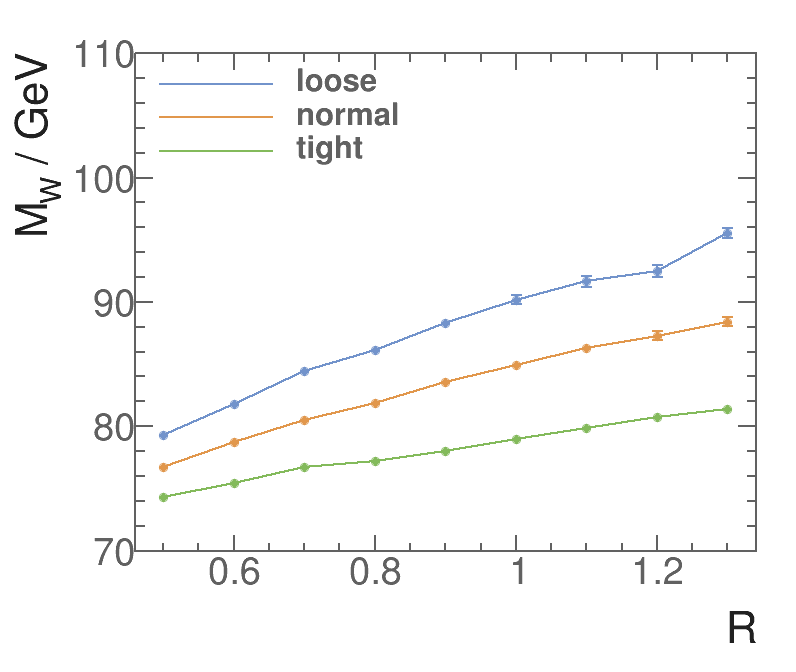
\includegraphics[width=\largefigwidth]{{{doubleHiggs/resolution/ILD_1.4TeV_W_M_testR}}} \\
\caption[Fitted mass, and resolution of \Hbb, \HWW and \PW for \rootS{1.4}]%
   {\Figure{fig:doubleHiggs1.4Higgs1M}, \ref{fig:doubleHiggs1.4Higgs2M}, and \ref{fig:doubleHiggs1.4WM}  show fitted mass of \Hbb, \HWW, and \PW, respectively, for loose, normal and tight selected PFO against $R$ parameter, with \rootS{1.4}. \Figure{fig:doubleHiggs1.4Higgs1Sigma}, \ref{fig:doubleHiggs1.4Higgs2Sigma}, and \ref{fig:doubleHiggs1.4WSigma} show fitted combined widths divided by the fitted masses of \Hbb, \HWW, and \PW, respectively, for loose, normal and tight selected PFO against $R$ parameter, with \rootS{1.4}.}
   \label{fig:doubleHiggs1.4TeVMassFit}
\end{figure}


For \rootS{3}, the choice is a bit more complicated. Shown in \Figure{fig:doubleHiggs3TeVMassFit}, fitted mass for \Hbb favours \normalPFO with $R = 0.8$. Fitted mass for \HWW favours \tightPFO with $R = 0.9$. Fitted mass for \PW favours \tightPFO with $R = 0.8$. Looking at the combined relative fitted width for the \Hbb, \HWW and \PW, shown in \Figure{fig:doubleHiggs3TeVSigmaFit}, \normalPFO gives a larger width than \tightPFO. Within \tightPFO, small $R$ values provide a shaper width for \HWW and \Hbb, but a broader width for \PW. Therefore, \tightPFO with $R = 0.7$ and $R = 1$ are both chosen for parallel analysis.

Later it was shown that \tightPFO with $R = 0.7$ gives a better signal significance. Therefore the optimal choice of jet reconstruction for \rootS{3} is \tightPFO with $R = 0.7$.

\begin{figure}[!tbp]
  \begin{subfigure}[b]{0.45\textwidth}
    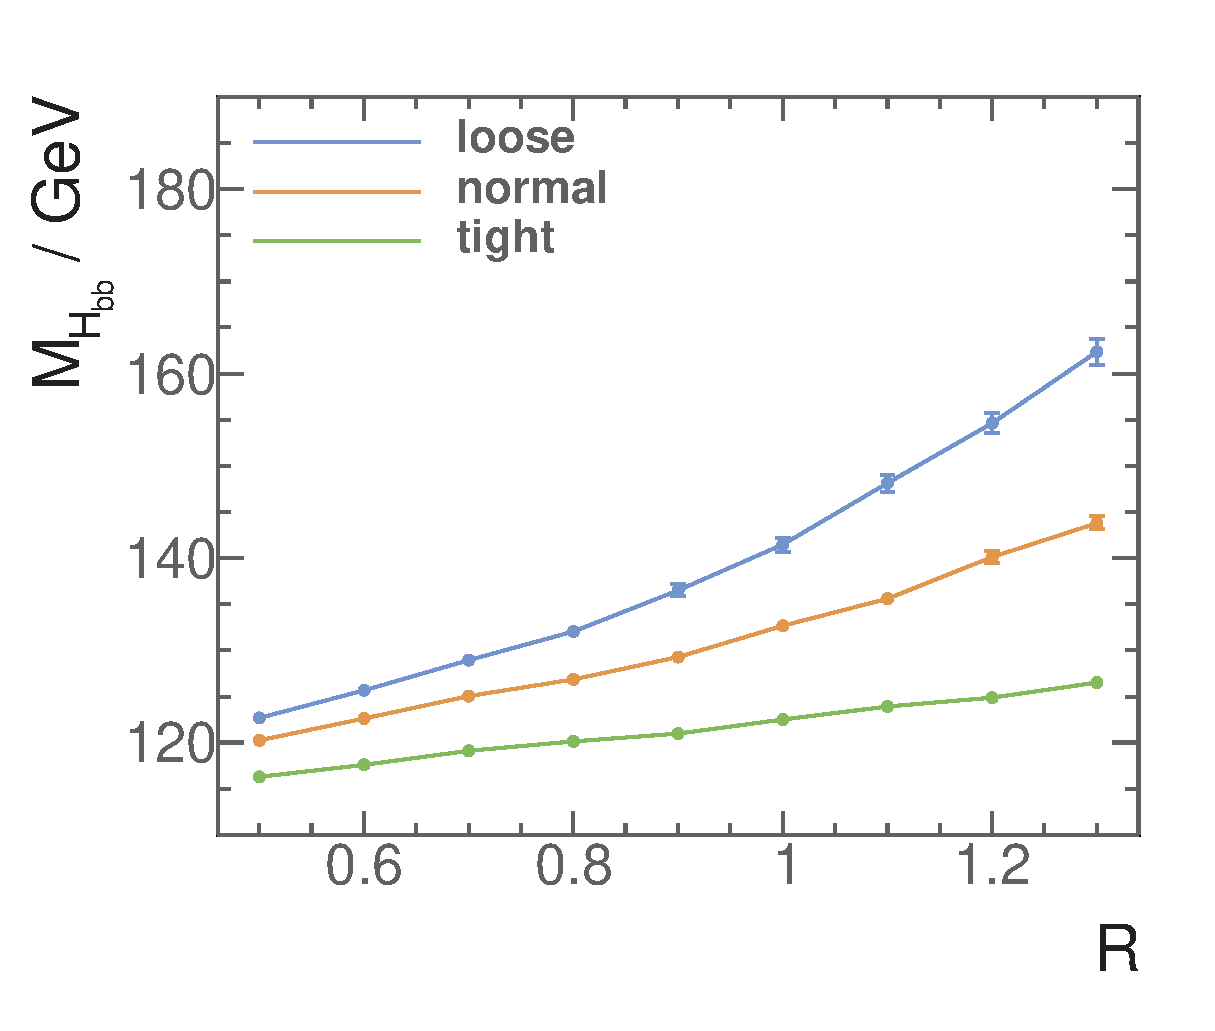
\includegraphics[width=\textwidth]{{{doubleHiggs/resolution/ILD_3TeV_Higgs1_M_R}}}
    \caption{}
    \label{fig:doubleHiggs3Higgs1M}
  \end{subfigure}
  \hfill
  \begin{subfigure}[b]{0.45\textwidth}
    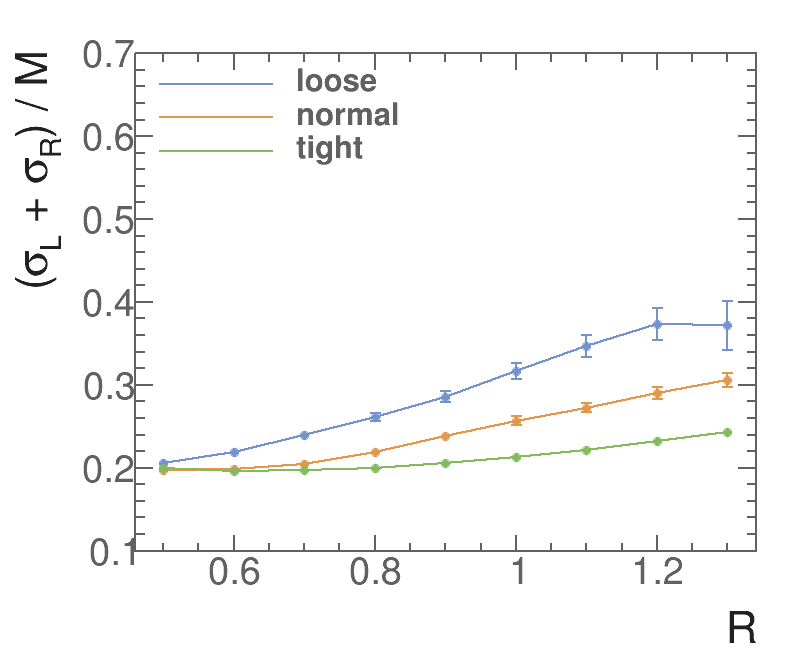
\includegraphics[width=\textwidth]{{{doubleHiggs/resolution/ILD_3TeV_Higgs1_SigmaL_add_SigmaR_divide_M_testR}}}
    \caption{}
    \label{fig:doubleHiggs3Higgs1Sigma}
  \end{subfigure}

  \begin{subfigure}[b]{0.45\textwidth}
    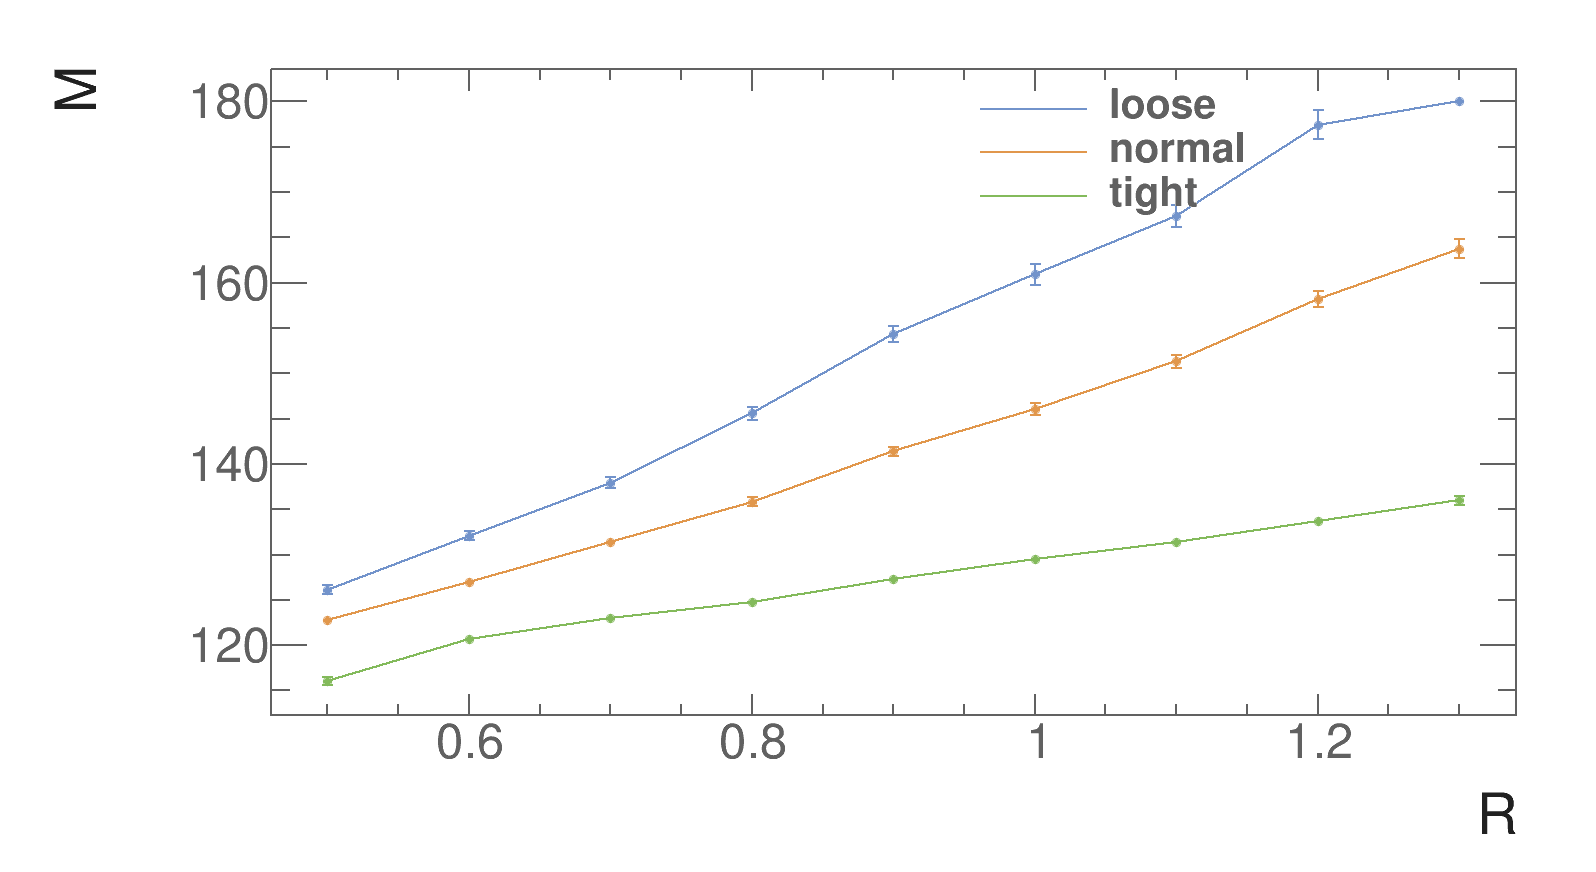
\includegraphics[width=\textwidth]{{{doubleHiggs/resolution/ILD_3TeV_Higgs2_M_R}}}
    \caption{}
    \label{fig:doubleHiggs3Higgs2M}
  \end{subfigure}
  \hfill
  \begin{subfigure}[b]{0.45\textwidth}
    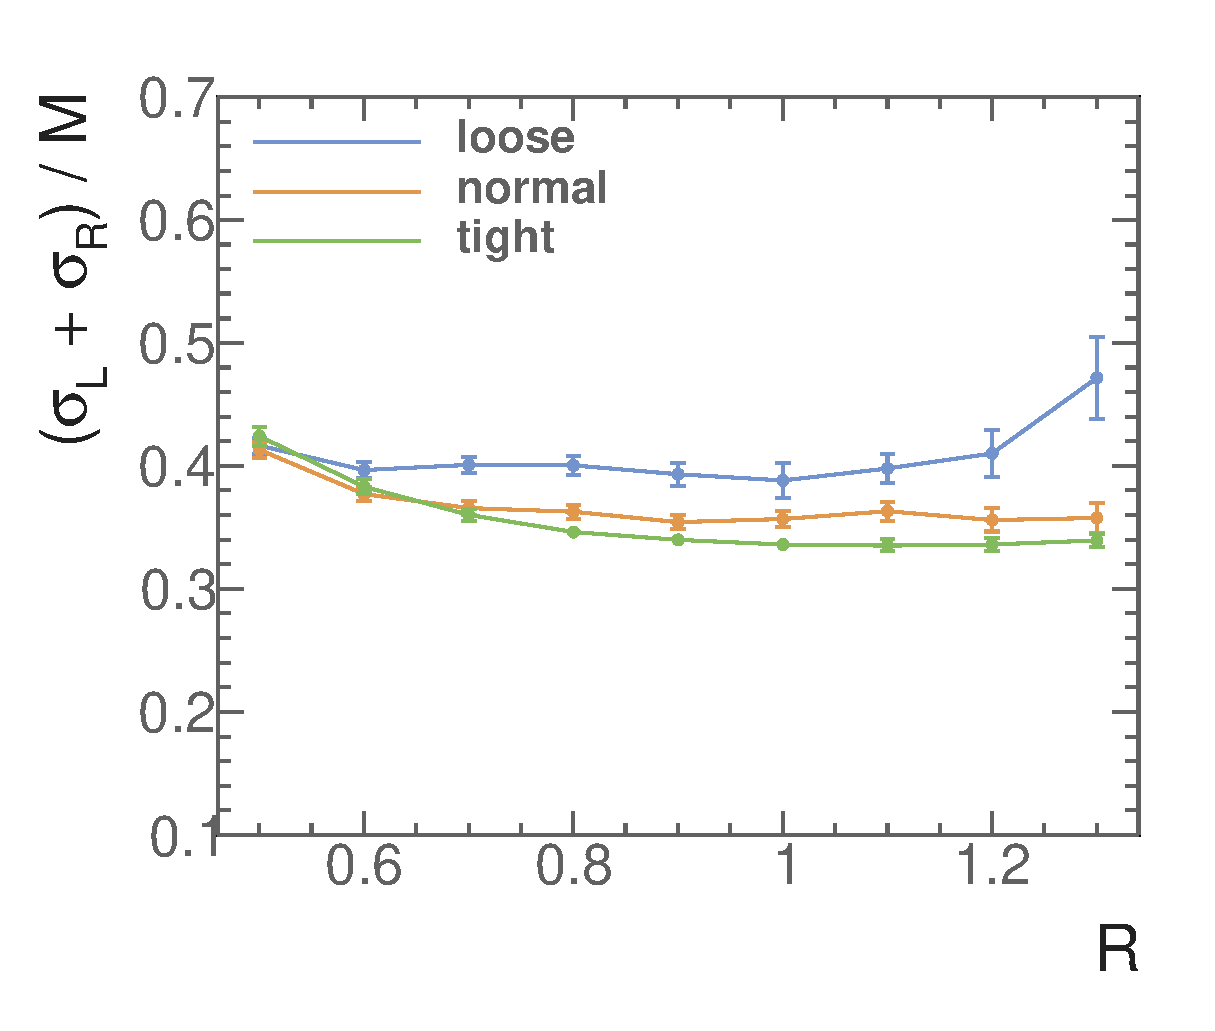
\includegraphics[width=\textwidth]{{{doubleHiggs/resolution/ILD_3TeV_Higgs2_SigmaL_add_SigmaR_divide_M_testR}}}
    \caption{}
    \label{fig:doubleHiggs3Higgs2Sigma}
  \end{subfigure}

  \begin{subfigure}[b]{0.45\textwidth}
    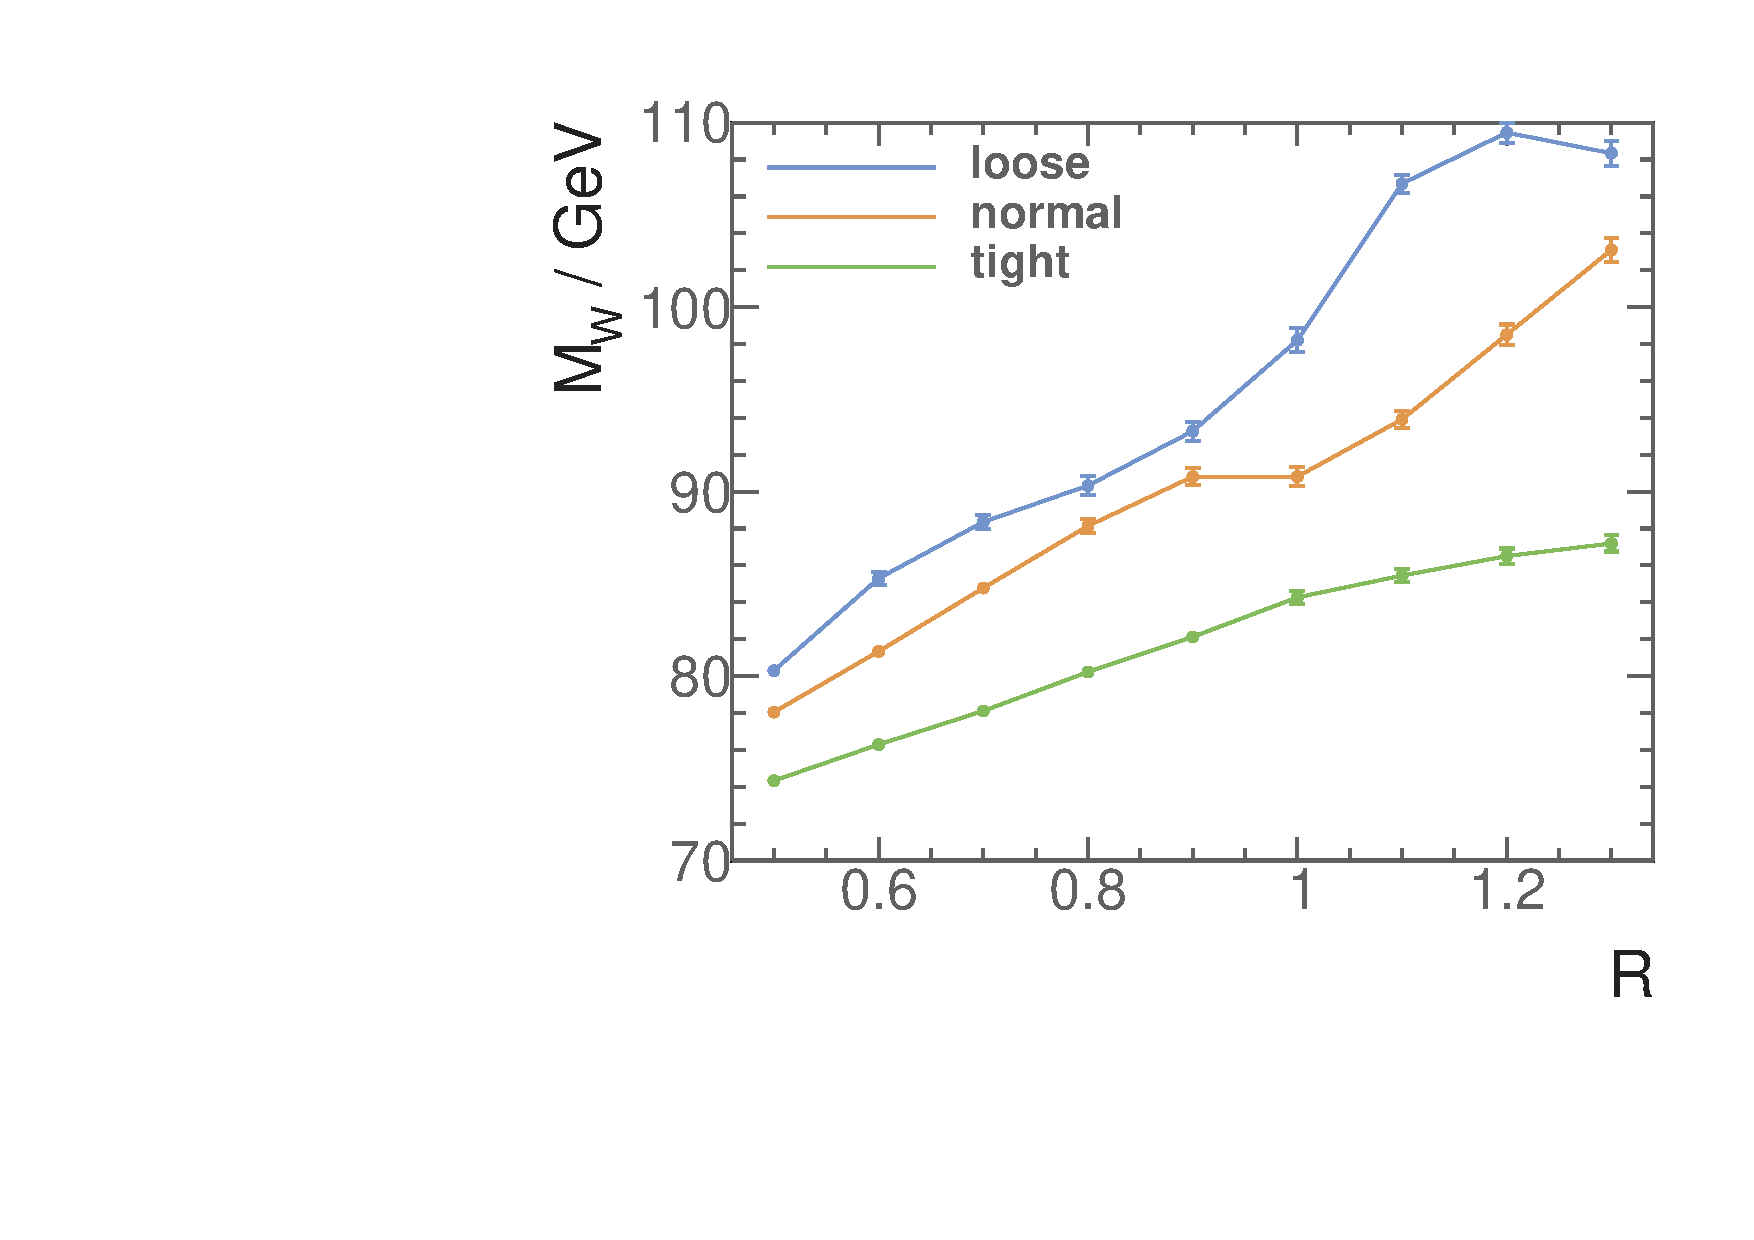
\includegraphics[width=\textwidth]{{{doubleHiggs/resolution/ILD_3TeV_W_M_testR}}}
    \caption{}
    \label{fig:doubleHiggs3WM}
  \end{subfigure}
  \hfill
  \begin{subfigure}[b]{0.45\textwidth}
    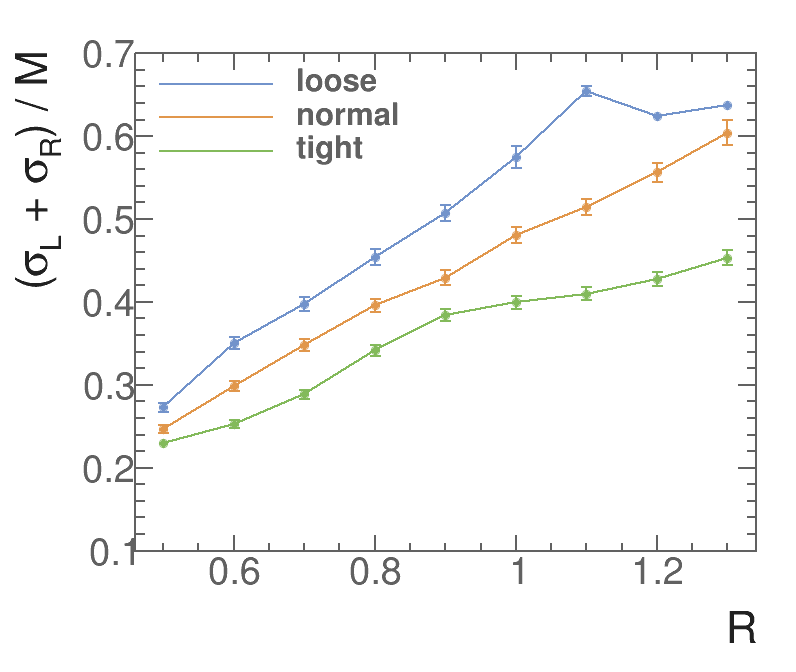
\includegraphics[width=\textwidth]{{{doubleHiggs/resolution/ILD_3TeV_W_SigmaL_add_SigmaR_divide_M_testR}}}
    \caption{}
    \label{fig:doubleHiggs3WSigma}
  \end{subfigure}

\caption[Fitted mass, and resolution of \Hbb, \HWW and \PW for \rootS{3}]%
   {\Figure{fig:doubleHiggs3Higgs1M}, \ref{fig:doubleHiggs3Higgs2M}, and \ref{fig:doubleHiggs3WM}  show fitted mass of \Hbb, \HWW, and \PW, respectively, for loose, normal and tight selected PFO against $R$ parameter, with \rootS{3}. \Figure{fig:doubleHiggs3Higgs1Sigma}, \ref{fig:doubleHiggs3Higgs2Sigma}, and \ref{fig:doubleHiggs3WSigma} show fitted combined widths divided by the fitted masses of \Hbb, \HWW, and \PW, respectively, for loose, normal and tight selected PFO against $R$ parameter, with \rootS{3}.}
   \label{fig:doubleHiggs3TeVMassFit}
\end{figure}


The extracted fitted parameters of optimal jet reconstructions are summarised in \Table{tab:doubleHiggsFitParameters}.


\begin{table}[!tbp]
\begin{tabular}{lrr}
\hline
\hline
Jet Parameters  &  \rootS{1.4} & \rootS{3}  \\
\hline
$\mu_{\Hbb}$ & $122.3_{\pm0.2}$ & $119.1_{\pm0.3}$  \\
$\sigma_{L,\Hbb}$ & $15.2_{\pm0.2}$ & $15.0_{\pm0.3}$  \\
$\sigma_{R,\Hbb}$ & $7.55_{\pm0.16}$ & $8.4_{\pm0.2}$  \\
\hline
$\mu_{\HWW}$ & $125.7_{\pm0.2}$ & $123.0_{\pm0.3}$  \\
$\sigma_{L,\HWW}$ & $29.4_{\pm0.3}$ & $36.6_{\pm0.6}$  \\
$\sigma_{R,\HWW}$ & $7.18_{\pm0.17}$ & $7.4_{\pm0.2}$  \\
\hline
$\mu_{\PW}$ & $80.5_{\pm0.2}$ & $78.1_{\pm0.3}$ \\
$\sigma_{L,\PW}$ & $16.2_{\pm0.3}$ & $13.1_{\pm0.4}$  \\
$\sigma_{R,\PW}$ & $9.03_{\pm0.16}$ & $9.5_{\pm0.2}$  \\
\hline
\hline
\end{tabular}
\caption
[The extracted fitted parameters of optimal jet reconstructions] %
{The extracted fitted parameters of optimal jet reconstructions, \normalPFO with $R = 0.7$ for \rootS{1.4} and \tightPFO with $R = 0.7$ for \rootS{3}.}
\label{tab:doubleHiggsFitParameters}
\end{table}

\begin{comment}
1996;n;0.7;Higgs1;122.32235414427674;15.240957200997611;7.5504561348187167;0.26543098613314636;0.12182184065528721;3113.2275806707034;0.22543433606291785;0.22430024486833489;0.15856304846729019;0.0030469485502088722;0.0032092877674692391;28.172240112940017;
1996;n;0.7;Higgs2;125.66836036851493;29.357519006393009;7.1835435253929738;0.060123174451423782;0.13449345831060805;2437.3997896140941;0.24231578716520374;0.3315313674793714;0.17355509758586773;0.0044154148101866499;0.0038407025785247018;20.405908034658069;
1996;n;0.7;W;80.53749728314051;16.232545245539399;9.0286457327628948;0.2207053340672821;0.11626433093587853;2979.6932364883933;0.21354250006439912;0.31981973411525555;0.1634330407590836;0.004577481212045903;0.0029533158186619834;32.462044237850932;

1998;t;0.7;Higgs1;119.13005080958837;15.037971702204626;8.3914897233789603;0.37671495896544804;0.12723226684850336;2450.6028763420195;0.29519717263163159;0.29538952246189165;0.20193802067306521;0.0041836006100050283;0.0039928785536029465;24.478700631527545;
1998;t;0.7;Higgs2;122.96923028319048;36.558655935687042;7.7126391897026139;0.093800035959964653;0.14914792076482761;1850.4313592700828;0.33028424129842904;0.566512280790338;0.22405806566158359;0.0077728968962250469;0.0042138236747335245;17.135754973108419;
1998;t;0.7;W;78.107124939496117;13.086676864110638;9.4516037466928928;0.47312266375623646;0.12798487896514332;2577.7712361437875;0.2531404220362532;0.39068260768287111;0.19051526092021209;0.0067777854263033344;0.0034288665863052362;31.161567527302168;

\end{comment}
\subsection{Jet flavour tagging}

Two b-jets out of six jets in \HepProcess final states are identified with flavour tagging processors. The processor calculates a set of discriminatively variables for a jet. After training the MVA, the MVA is applied to jets to produce a likelihood for b-jet and c-jet. For details see \Section{}.

The existing LCFIPlus processor in Marlin package is used. The training sample of the flavour tagging processor is \HepProcess{\Pem \Pep \to \PZ \Pnu \APnu}, where \PZ decays to \HepProcess{\qlight\Aqlight}, \HepProcess{\Pbottom\APbottom}, or \HepProcess{\Pcharm\APcharm} at \rootS{1.4} and \rootS{3}, because they have similar event topology as the signal, and they have only two jets in the final state.

The selection efficiency of b-jets and c-jets with trainning samples are shown in \Figure{}. Flavour tagging performs better at low energy. Because at high energy, particles at more collimated and more difficult to separate.

\begin{figure}[!tbp]
  \begin{subfigure}[b]{0.45\textwidth}
    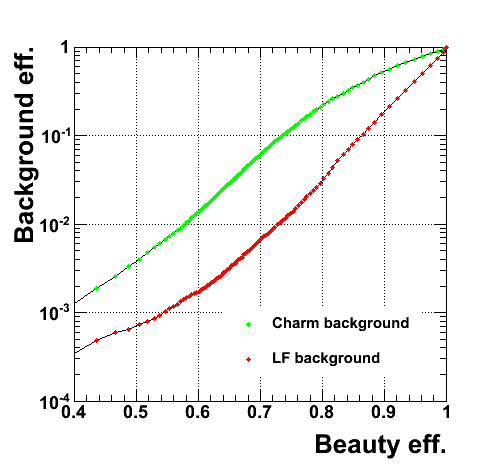
\includegraphics[width=\textwidth]{{{doubleHiggs/eval-lcfiweights_R0_7_2jets-test}}}
    \caption{\rootS{1.4}}
    \label{fig:doubleHiggs1.4Btag}
  \end{subfigure}
  \hfill
  \begin{subfigure}[b]{0.45\textwidth}
    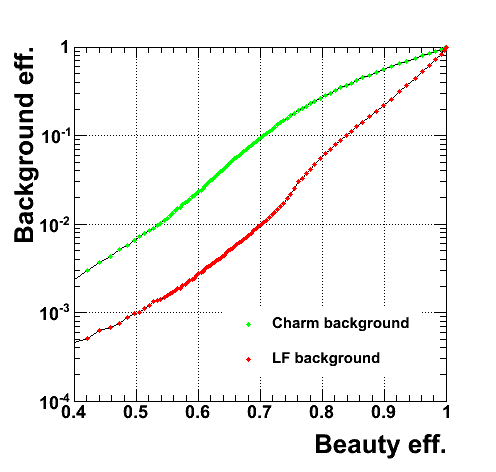
\includegraphics[width=\textwidth]{{{doubleHiggs/eval-lcfiweights_tR0_7_3000_2jets-test}}}
    \caption{\rootS{3}}
    \label{fig:doubleHiggs3Btag}
  \end{subfigure}
    \caption[Performance of b-jet tagging with trainning samples]%
   {Performance of b-jet tagging with trainning samples}
   \label{fig:doubleHiggsBtag}
\end{figure}

\subsection{Jet pairing}

The jet pairing was performed by checking combination of jets that are compatible with signal \eeToHHbbWW.

The actual pairing is done via a minimisation
\begin{equation}
	\chi^2 = \left(\frac{m_{ij}-\mu_{\Hbb}}{\sigma_{\Hbb}^{\prime}}\right)^2 + \left(\frac{m_{klmn}-\mu_{\HWW}}{\sigma_{\HWW}^{\prime}}\right)^2  + \left(\frac{m_{kl}-\mu_{\PW}}{\sigma_{\PW}^{\prime}}\right)^2,
%\label{eqn:eq_chi2_HHWWbb}
\end{equation}
where, $\mu_{\Hbb}$ and $\sigma_{\Hbb}^{\prime}$ are the fitted invariant mass, and the fitted width, respectively. Both are obtained in \Section{sec:doubleHiggsJetOptimisation}. $\sigma_{\Hbb}^{\prime}$ is $\sigma_{L,\Hbb}$ when $m_{ij} < m_{\Hbb}$, and $\sigma_{R,\Hbb}$ otherwise. Similarly $\mu_{\HWW}$ and $\mu_{\PW}$ are fitted mass, and $\sigma_{\HWW}^{\prime}$ and $\sigma_{\PW}^{\prime}$ are fitted invariant mass, and the fitted width, respectively. Out of the six jets from the jet clustering, indicated by subscript $i,j,k,l,m,n$, two are used for \Hbb, two for \PW and four for \HWW. The fitted parameters used are listed in \Table{tab:doubleHiggsFitParameters}. Additional requirement is that at least one of two jets forming \Hbb needs to have a b-jet tag of 0.2 or greater.

With the $\chi^2$, all possible combinations are tested, and the one with smallest $\chi^2$ is chosen.

\section{Pre-selection}

Discriminative variables were calculated. Some are used as to discard background events, whilst hurting the signal events a bit. This allows MVA to concentrate on events where it is difficult to separate in a single parameter space.

\subsection{Discriminative pre-selection cuts}

As discussed before, events with identified leptons are rejected. Jet pairing implies that events with the largest b-jet tag  less than 0.2 are rejected.

For \rootS{1.4}, a range of variables were tested and three where chosen as pre-selection cuts.

Event with invariant mass of two higgs less than 150\,GeV is rejected. The cut above 120\,GeV is needed as some background samples were generated only for invariant mass greater than 120\,GeV. Shown in \Table{} and \Figure{}, this cut is effective against samples with two quark final states.

Event with second highest b-jet tag less than 0.2 is rejected. This stricter cut than the jet pairing helps to reduce samples with no b-jets.

Event with \pT of two higgs less than 30\,GeV is rejected. This is extremely effective against samples with no neutrinos in the final state.

\begin{figure}[!tbp]
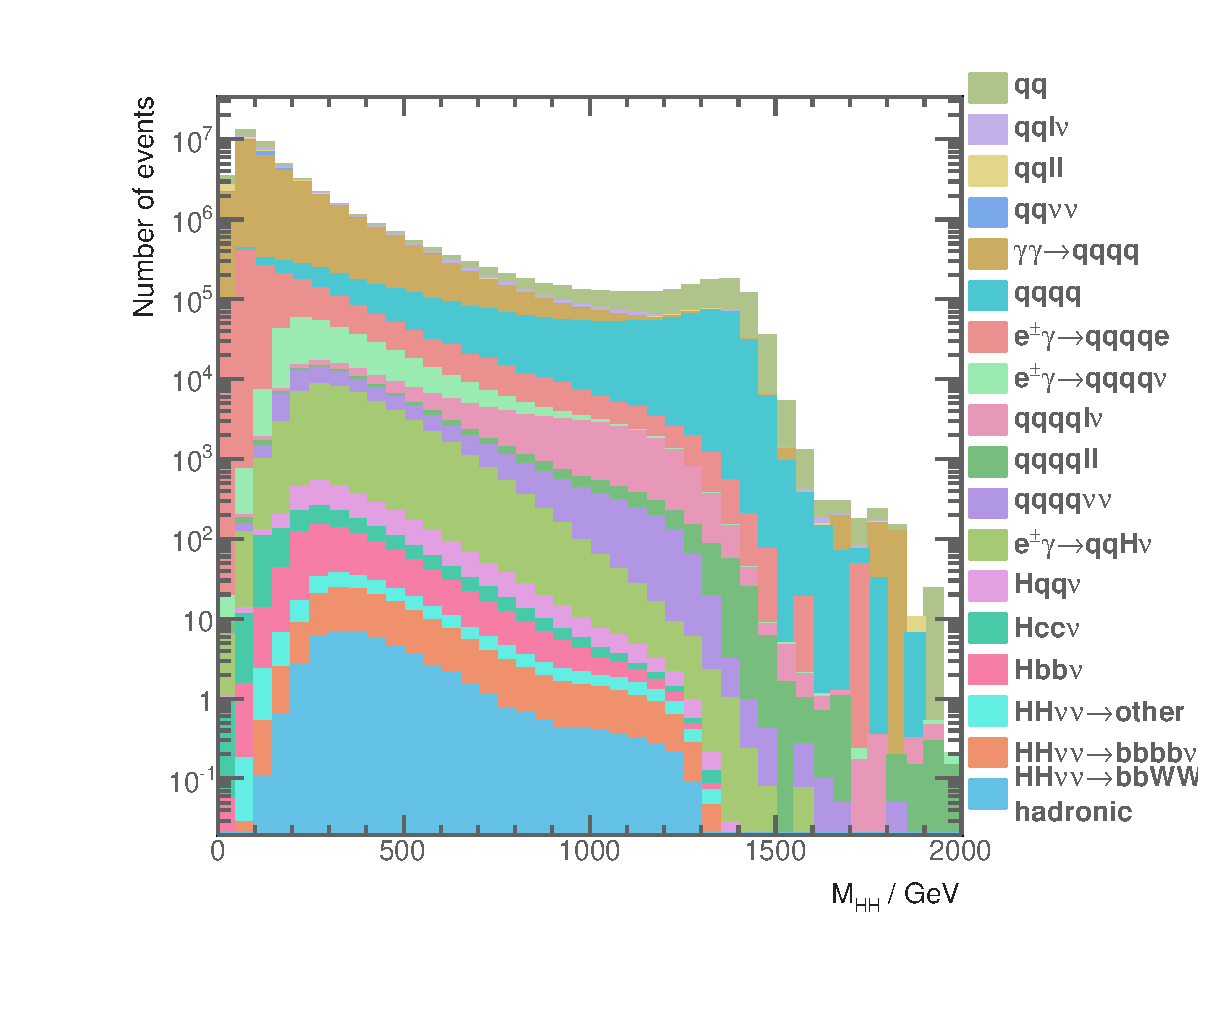
\includegraphics[width=\largefigwidth]{{{doubleHiggs/var/nR0_7_6jet_btag2_Higgs_all_M_TMVA20161208R0_7_qq_btag2_prepare}}} \\
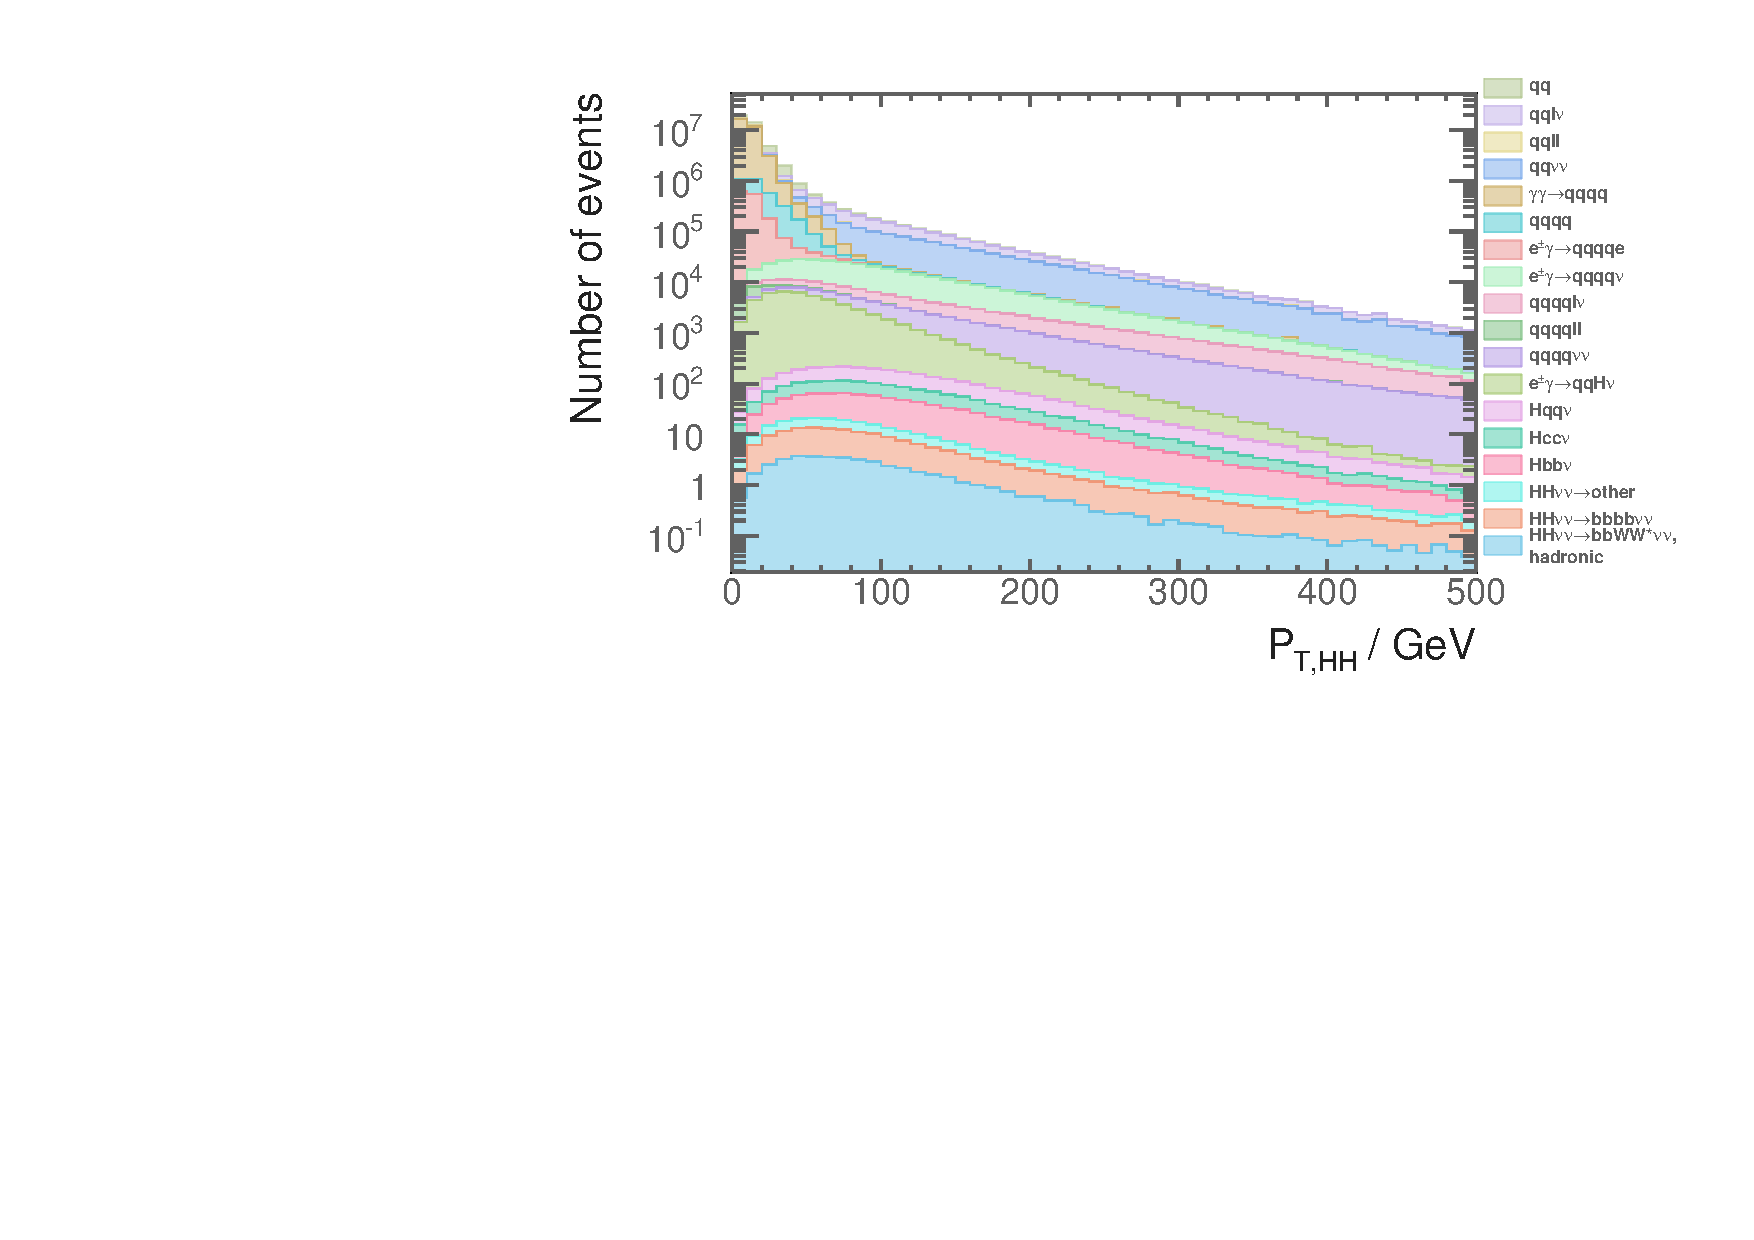
\includegraphics[width=\largefigwidth]{{{doubleHiggs/var/nR0_7_6jet_btag2_Higgs_all_Pt_TMVA20161208R0_7_qq_btag2_prepare}}} \\
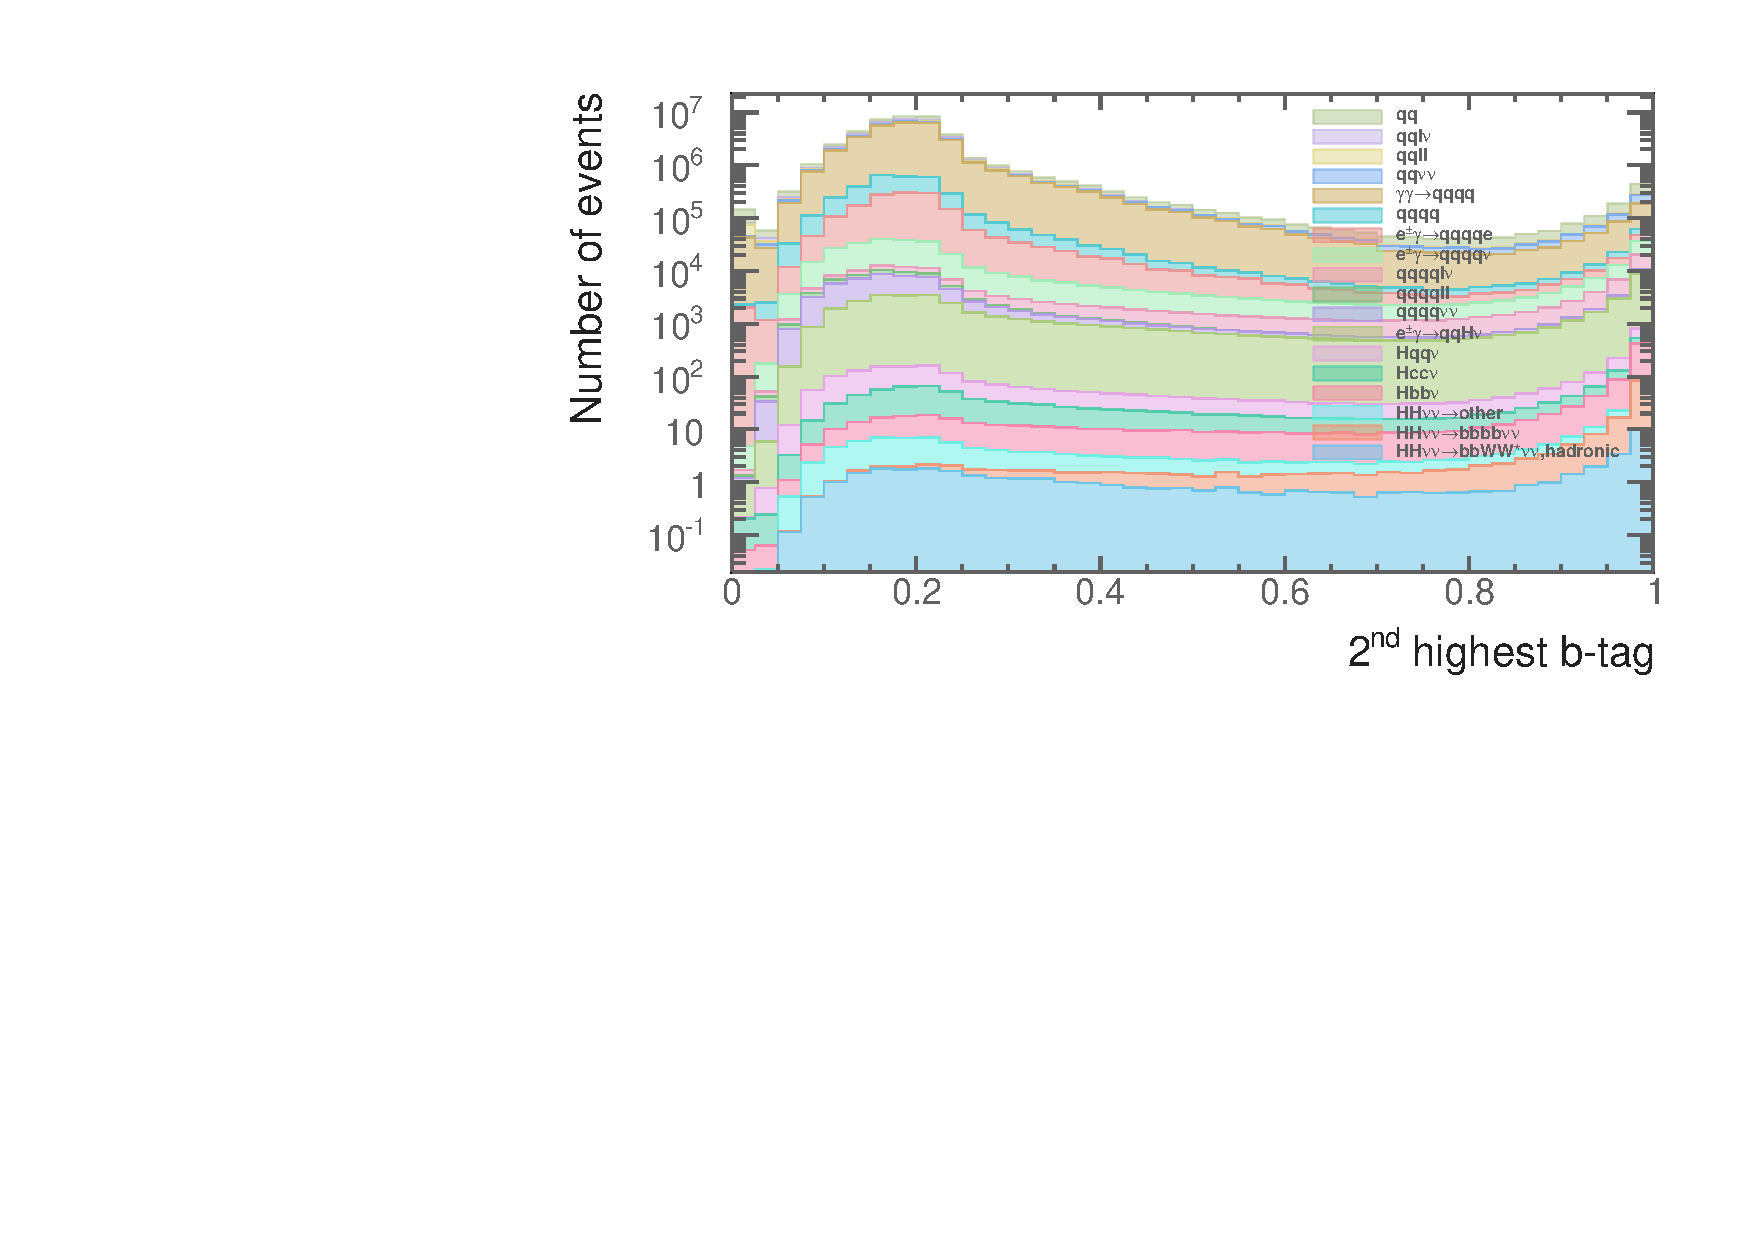
\includegraphics[width=\largefigwidth]{{{doubleHiggs/var/nR0_7_6jet_btag2_bTag2_TMVA20161208R0_7_qq_btag2_prepare}}} \\
\caption[Discriminative pre-selection variables for \rootS{1.4}]%
   {Discriminative pre-selection variables for \rootS{1.4}, after rejecting events with identified leptons, and jet pairing}
   \label{fig:doubleHiggs1.4TeVPreSelection}
\end{figure}

For \rootS{3}, event with invariant mass of two higgs less than 150\,GeV is rejected, for the reason similar to \rootS{1.4}.

In addition, event with highest b-jet tag less than 0.7 is rejected. It is found that b-jet tag is less efficient at a higher \sqrtS. Therefore, a stricter cut at b-jet tag is useful to compensate for the tagging efficiency loss.

\begin{figure}[!tbp]
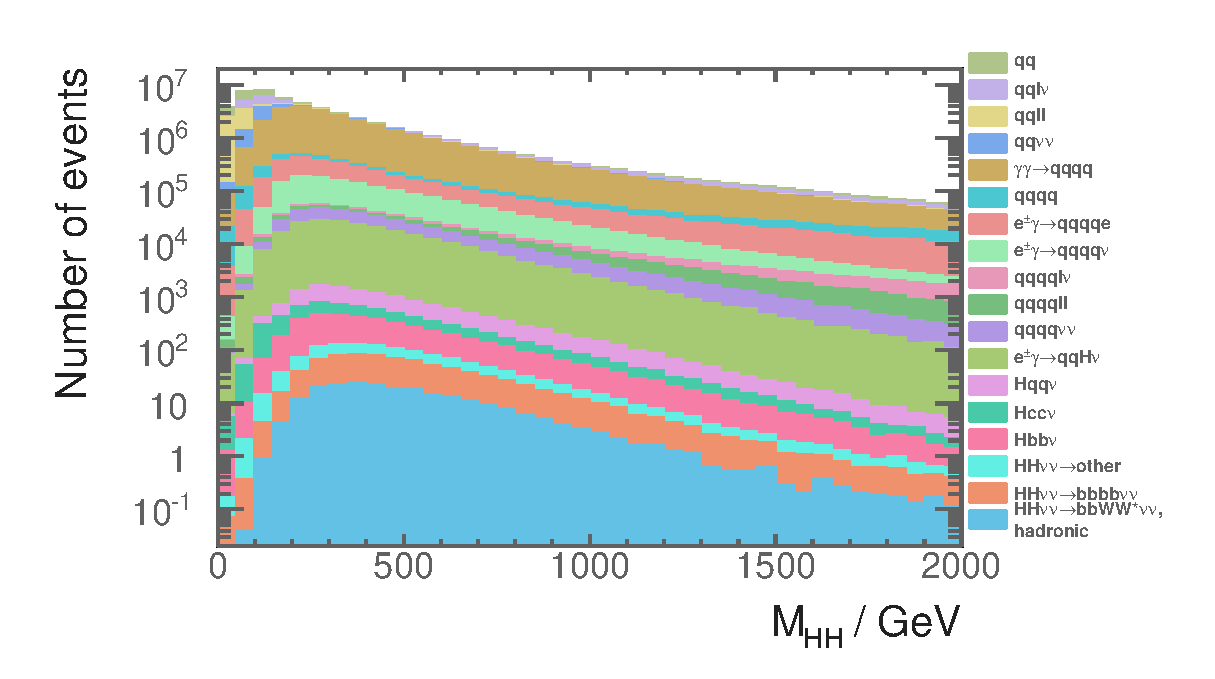
\includegraphics[width=\largefigwidth]{{{doubleHiggs/var/tR0_7_6jet_btag2_Higgs_all_M_TMVA201612083TeVtR0_7_qq_btag2_prepare}}} \\
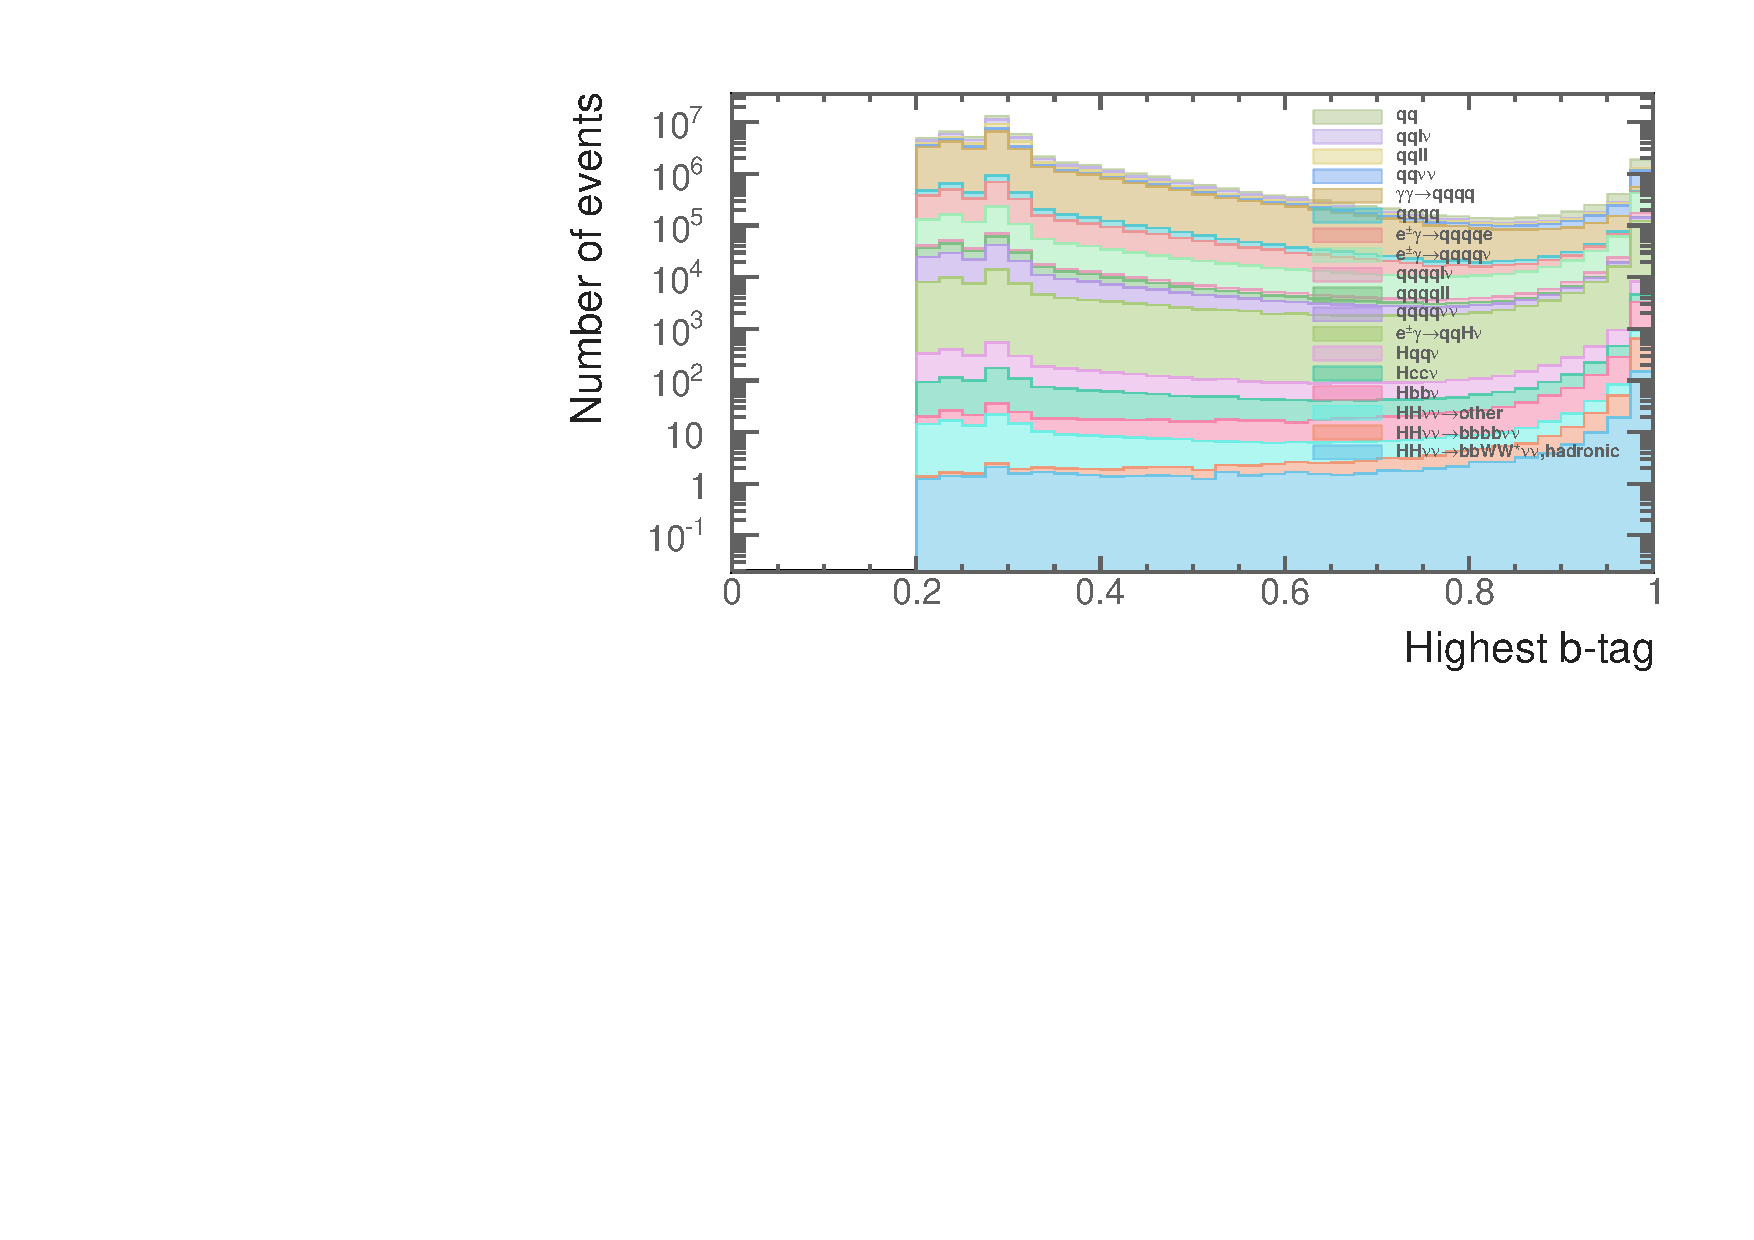
\includegraphics[width=\largefigwidth]{{{doubleHiggs/var/tR0_7_6jet_btag2_bTag1_TMVA201612083TeVtR0_7_qq_btag2_prepare}}} \\
\caption[Discriminative pre-selection variables for \rootS{3}]%
   {Discriminative pre-selection variables for \rootS{3}, after rejecting events with identified leptons, and jet pairing}
   \label{fig:doubleHiggsTeVPreSelection}
\end{figure}



These set of cuts are stricter than usual analysis. The cross sections of signal channel for both \sqrtS are extremely small, comparing to the background. Hence only the signal events with very clear characteristic topologies would be able to pass the final selection, in order to achieve a decent signal-to-background ratio. Therefore, a strict pre-selection cut would not hurt the final signal selection. On the contrary, final signal selection would benefit from MVA being able to focus the difficult background events, where their topologies are too similar to the signal events to separate in any single parameter space.

\begin{table}[!tbp]\centering
% TODO fix lumi correction for e gamma, gamma e
% TODO change some of sample cross section for  electron-photon interaction with four quarks and a neutrino final state
%\small{
\small
\begin{tabular}{lrrrrr}
\hline \hline
 \multicolumn{1}{m{3.5cm}}{Channel / Efficiency \rootS{1.4}} &  \multicolumn{1}{m{2cm}}{Expected number of events}  & \multicolumn{1}{m{2cm}}{Lepton ID and jet pairing} & \multicolumn{1}{m{1.5cm}}{$m_{HH}>150\xspace{GeV}$} & \multicolumn{1}{m{1.5cm}}{$B_{2}>0.2$} & \multicolumn{1}{m{1.5cm}}{$\Pt>30\xspace{GeV}$}  \\
\hline
\eeToHH $\to$ \\
\HepProcess{ \Pbottom \APbottom \PWplus \PWminus \Pnu \APnu}, hadronic             &27.9& 85.8\% & 85.6\% & 73.7\%& 66.4\%\\
\hline
\eeToHH $\to$ \\
\HepProcess{ \Pbottom \APbottom \Pbottom \APbottom \Pnu \APnu}             &67.6& 90.8\% & 90.5\% & 90.1\% & 80.6\%\\
\eeToHH $\to$ other & 128.0 & 36.2\% & 35.3\% & 27.7\% & 24.7\%\\
\hline
\eeTo{\qlight \qlight \PHiggs \Pnu \APnu}  & 1304.0 & 60.7\% & 59.8\% & 44.9\%& 42.0\%\\
\eeTo{\Pcharm \APcharm \PHiggs \Pnu \APnu}  & 546.1 & 67.4\%& 57.7\%& 46.5\%& 43.4\%\\
\eeTo{\Pbottom \APbottom \PHiggs \Pnu \APnu}  & 463.0 & 73.9\%& 72.6\%& 68.7\%& 64.2\%\\

\eeTo{ \Pquark \Pquark \Pquark \Pquark}   &   1867650.0& 48.8\% & 46.1\%& 17.3\%& 4.7\%\\
\eeTo{ \Pquark \Pquark \Pquark \Pquark \Plepton \Plepton}& 93150.0 & 5.0\%& 4.9\%& 1.5\%& 0.3\%\\
\eeTo{ \Pquark \Pquark \Pquark \Pquark \Plepton \Pnu}& 165600.0 & 15.1\%& 15.1\%& 12.4\%& 11.4\%\\
\eeTo{ \Pquark \Pquark \Pquark \Pquark \Pnu \APnu} & 34800.0& 50.7\%& 50.0\%& 20.1\%& 18.8\%\\

\eeTo{ \Pquark \Pquark} &  6014250.0 & 54.5\%& 17.5\%& 8.4\%& 2.2\%\\
\eeTo{ \Pquark \Pquark \Plepton \Pnu} &  6464550.0 & 14.1\%& 5.3\%& 2.0\%& 1.6\%\\
\eeTo{ \Pquark \Pquark \Pl \Pl} &  4088700.0 & 13.0\%& 1.1\%& 0.6\%& 0.1\%\\
\eeTo{ \Pquark \Pquark \Pnu \Pnu} & 1181550.0 & 60.1\%& 12.3\%& 6.2\%& 5.8\% \\
\hline
\egamma{\Pem}{\Pphoton}{BS}{\Pem \Pquark \Pquark \Pquark \Pquark} & 1305787.5  & 23.3\%& 10.6\%& 4.4\%& 0.4\%\\
\egamma{\Pep}{\Pphoton}{BS}{\Pep \Pquark \Pquark \Pquark \Pquark} & 1300837.5 & 23.4\%& 10.5\%& 4.3\%& 0.4\%\\
\egamma{\Pem}{\Pphoton}{EPA}{\Pem \Pquark \Pquark \Pquark \Pquark} & 430650.0 & 11.1\%& 5.4\%& 2.2\%& 0.3\%\\
\egamma{\Pep}{\Pphoton}{EPA}{\Pep \Pquark \Pquark \Pquark \Pquark}  & 430350.0 & 11.1\% & 5.3\%& 2.1\%& 0.3\%\\
\egamma{\Pem}{\Pphoton}{BS}{\Pnu \Pquark \Pquark \Pquark \Pquark}& 89775.0  & 58.3\%& 56.8\%& 31.0\%& 27.7\%\\
\egamma{\Pep}{\Pphoton}{BS}{\APnu \Pquark \Pquark \Pquark \Pquark}& 89212.5 & 57.6\% & 56.1\%& 30.3\%& 27.3\%\\
\egamma{\Pem}{\Pphoton}{EPA}{\Pnu \Pquark \Pquark \Pquark \Pquark}& 26100.0  & 29.6\% & 28.9\%& 15.4\%& 13.9\%\\
\egamma{\Pep}{\Pphoton}{EPA}{\APnu \Pquark \Pquark \Pquark \Pquark}& 25950.0  & 29.2\%& 28.5\%& 15.0\% & 13.7\%\\

\egamma{\Pem}{\Pphoton}{BS}{\Pquark \Pquark \PHiggs \Pnu} & 17775  & 61.0\% & 59.8\%& 45.5\%& 34.6\%\\
\egamma{\Pep}{\Pphoton}{BS}{\Pquark \Pquark \PHiggs \Pnu} & 17662.5  & 61.1\% & 60.0\% & 45.6\% & 34.6\%\\
\egamma{\Pem}{\Pphoton}{EPA}{\Pquark \Pquark \PHiggs \Pnu} & 5085  & 31.8\% & 31.2\% & 23.7\%& 18.2\%\\
\egamma{\Pep}{\Pphoton}{EPA}{\Pquark \Pquark \PHiggs \Pnu} & 5085   & 31.9\% & 31.3\% & 23.8\% & 18.4\%\\
\hline
\gammagamma{\Pphoton}{BS}{\Pphoton}{BS}{ \Pquark \Pquark \Pquark \Pquark}& 2054951.5  & 56.3\%& 23.9\%& 9.6\%& 0.3\%\\
\gammagamma{\Pphoton}{BS}{\Pphoton}{EPA}{ \Pquark \Pquark \Pquark \Pquark}& 4521037.5  &33.6\%& 14.2\%& 5.7\%& 0.4\%\\
\gammagamma{\Pphoton}{EPA}{\Pphoton}{BS}{ \Pquark \Pquark \Pquark \Pquark}& 4539150.0 & 33.7\%& 14.2\%& 5.7\%& 0.4\%\\
\gammagamma{\Pphoton}{EPA}{\Pphoton}{EPA}{ \Pquark \Pquark \Pquark \Pquark}& 1129500.0 & 21.1\% & 9.1\% & 3.7\%& 0.4\%\\
\hline \hline
\end{tabular}

\caption{List of signal and background samples with the corresponding expected number at  \rootS{1.4}, assuming a luminosity of 1500$fb^{-1}$. The selection efficiencies are presented in a ``flow'' fashion, as the every selection cut contains all the cuts to the left of it.
}
\label{tab:doubleHiggs1.4TeVPreslection}
\end{table}

\begin{table}[!tbp]\centering
% TODO fix lumi correction for e gamma, gamma e
% TODO change some of sample cross section for  electron-photon interaction with four quarks and a neutrino final state
%\small{
\small
\begin{tabular}{lrrrr}
\hline \hline
 \multicolumn{1}{m{3.5cm}}{Channel / Efficiency \rootS{3}} &  \multicolumn{1}{m{2cm}}{Expected number of events}  & \multicolumn{1}{m{2cm}}{Lepton ID and jet pairing} & \multicolumn{1}{m{1.5cm}}{$m_{HH}>150\xspace{GeV}$} & \multicolumn{1}{m{1.5cm}}{$B_{1}>0.7$} \\
\hline
\eeToHH $\to$ \\
\HepProcess{ \Pbottom \APbottom \PWplus \PWminus \Pnu \APnu}, hadronic             &146.0& 80.2\% & 79.9\% & 69.7\%\\
\hline
\eeToHH $\to$ \\
\HepProcess{ \Pbottom \APbottom \Pbottom \APbottom \Pnu \APnu}             &355.0& 83.4\% & 82.9\% & 81.2\% \\
\eeToHH $\to$ other & 675.0 & 36.7\% & 35.8\% & 25.2\% \\
\hline
\eeTo{\qlight \qlight \PHiggs \Pnu \APnu}  & 6115.4 & 59.5\% & 58.5\% & 40.4\%\\
\eeTo{\Pcharm \APcharm \PHiggs \Pnu \APnu}  & 2249.9 & 64.8\%& 58.4\%& 39.3\%\\
\eeTo{\Pbottom \APbottom \PHiggs \Pnu \APnu}  & 2197.7 & 69.7\%& 68.4\%& 64.2\%\\

\eeTo{ \Pquark \Pquark \Pquark \Pquark}   &   1093000.0& 48.5\% & 39.7\%& 3.0\%\\
\eeTo{ \Pquark \Pquark \Pquark \Pquark \Plepton \Plepton}& 338600.0 & 14.7\%& 14.2\%& 0.7\%\\
\eeTo{ \Pquark \Pquark \Pquark \Pquark \Plepton \Pnu}& 213200.0 & 19.7\%& 19.4\%& 10.0\%\\
\eeTo{ \Pquark \Pquark \Pquark \Pquark \Pnu \APnu} & 143000.0& 58.4\%& 57.3\%& 11.9\%\\

\eeTo{ \Pquark \Pquark} &  5897800.0 & 62.8\%& 13.2\%& 2.7\%\\
\eeTo{ \Pquark \Pquark \Plepton \Pnu} &  11121800 & 28.3\%& 11.9\%& 0.3\%\\
\eeTo{ \Pquark \Pquark \Pl \Pl} &  6639200.0 & 38.3\%& 2.9\%& 0.7\%\\
\eeTo{ \Pquark \Pquark \Pnu \Pnu} & 2635000.0 & 71.4\%& 24.1\%& 5.3\% \\
\hline
\egamma{\Pem}{\Pphoton}{BS}{\Pem \Pquark \Pquark \Pquark \Pquark} & 2004388.1  & 23.3\%& 21.5\%& 0.8\%\\
\egamma{\Pep}{\Pphoton}{BS}{\Pep \Pquark \Pquark \Pquark \Pquark} & 2002334.1 & 23.4\%& 21.6\%& 0.8\%\\
\egamma{\Pem}{\Pphoton}{EPA}{\Pem \Pquark \Pquark \Pquark \Pquark} & 575600.0& 12.0\%& 11.0\%& 0.5\%\\
\egamma{\Pep}{\Pphoton}{EPA}{\Pep \Pquark \Pquark \Pquark \Pquark}  & 575600.0 & 12.0\% & 10.9\%& 0.4\%\\
\egamma{\Pem}{\Pphoton}{BS}{\Pnu \Pquark \Pquark \Pquark \Pquark}& 414750.0  & 61.7\%& 59.5\%& 20.4\%\\
\egamma{\Pep}{\Pphoton}{BS}{\APnu \Pquark \Pquark \Pquark \Pquark}& 414434.0 & 61.2\% & 59.1\%& 19.4\%\\
\egamma{\Pem}{\Pphoton}{EPA}{\Pnu \Pquark \Pquark \Pquark \Pquark}& 108400.0  & 30.9\% & 29.9\%& 9.6\%\\
\egamma{\Pep}{\Pphoton}{EPA}{\APnu \Pquark \Pquark \Pquark \Pquark}& 108400.0  & 30.7\%& 29.7\%& 9.1\% \\

\egamma{\Pem}{\Pphoton}{BS}{\Pquark \Pquark \PHiggs \Pnu} & 92588.0  & 58.3\% &56.2\%& 37.3\% \\
\egamma{\Pep}{\Pphoton}{BS}{\Pquark \Pquark \PHiggs \Pnu} & 92430.0 & 58.1\% & 56.0\% & 37.1\% \\
\egamma{\Pem}{\Pphoton}{EPA}{\Pquark \Pquark \PHiggs \Pnu} & 23400.0 & 30.1\% &29.2\% & 19.4\% \\
\egamma{\Pep}{\Pphoton}{EPA}{\Pquark \Pquark \PHiggs \Pnu} & 23400.0   & 29.7\% & 28.6\% & 18.8\% \\
\hline
\gammagamma{\Pphoton}{BS}{\Pphoton}{BS}{ \Pquark \Pquark \Pquark \Pquark}& 18009413.9  & 54.2\%& 49.2\%& 1.9\%\\
\gammagamma{\Pphoton}{BS}{\Pphoton}{EPA}{ \Pquark \Pquark \Pquark \Pquark}& 3824548.1  &33.5\%& 30.2\%& 1.2\%\\
\gammagamma{\Pphoton}{EPA}{\Pphoton}{BS}{ \Pquark \Pquark \Pquark \Pquark}& 3828498.1 & 33.7\%& 30.3\%& 1.2\%\\
\gammagamma{\Pphoton}{EPA}{\Pphoton}{EPA}{ \Pquark \Pquark \Pquark \Pquark}& 805400.0 & 22.0\% & 19.8\% & 0.8\%\\
\hline \hline
\end{tabular}

\caption{List of signal and background samples with the corresponding expected number at \rootS{3}, assuming a luminosity of 2000$fb^{-1}$. The selection efficiencies are presented in a ``flow'' fashion, as the every selection cut contains all the cuts to the left of it.
}
\label{tab:doubleHiggs1.4TeVPreslection}
\end{table}


\subsection{Sanity cuts}

A set of very loose cuts, aiming to reduce the range of some discriminative variables to increase the effectiveness of MVA. (See \Section{} on MVA) These cuts are very loose and physics motivated.

For \rootS{1.4}, invariant masses for \Hbb, \HWW, \PW, and \HH are smaller than 500, 800, 200, and 1400\,GeV, respectively.

For \rootS{3}, invariant masses for \Hbb, \HWW, \PW, and \HH are smaller than 500, 800, 200, and 3000\,GeV, respectively.

The selection efficiencies after sanity cuts and other pre-selection cuts stated above, are listed in \Table{}.

\subsection{Mutually exclusive cuts for \eeToHHbbWW and \eeToHHbbbb}

Since the analysis for \eeToHH channel is divided into two subchannels, \eeToHHbbWWHad and \eeToHHbbbb, it is convenient to divided samples, both signal and background, into two mutually exclusive sets. This will make combining subchaneels much easier, as correlations between subchannels do not need to be considered.

The most distinctive difference between two subchannels, is that they have different number of jets, and different number of b-jets in the final state. So variables related to number of b-jets or a number of jets are suitable for separating two subchannels.

Shown in \Figure{fig:doubleHiggsMutualPreselection}, two subchannels can be clearly separated in the two dimensional parameter space. The optimal rectangular cuts were selected by scanning the two parameters, and maximising
\begin{equation}
\varepsilon = P(subchannel_1|selection) \times P(subchannel_2|\neg{selection})
\end{equation}
where $selection$ represents the mutually exclusive cuts, $\neg{selection}$ indicates the phase space not covered by the $selection$.

Variables tested includes \sumBtag{4}, \partialSumBtag{1}{3}{4}, \y{34}, \y{45}, \y{56}, \y{67} and other related variables. The best separation was summarised in \Table{tab:doubleHiggsMutualCuts}.

\begin{figure}[!tbp]
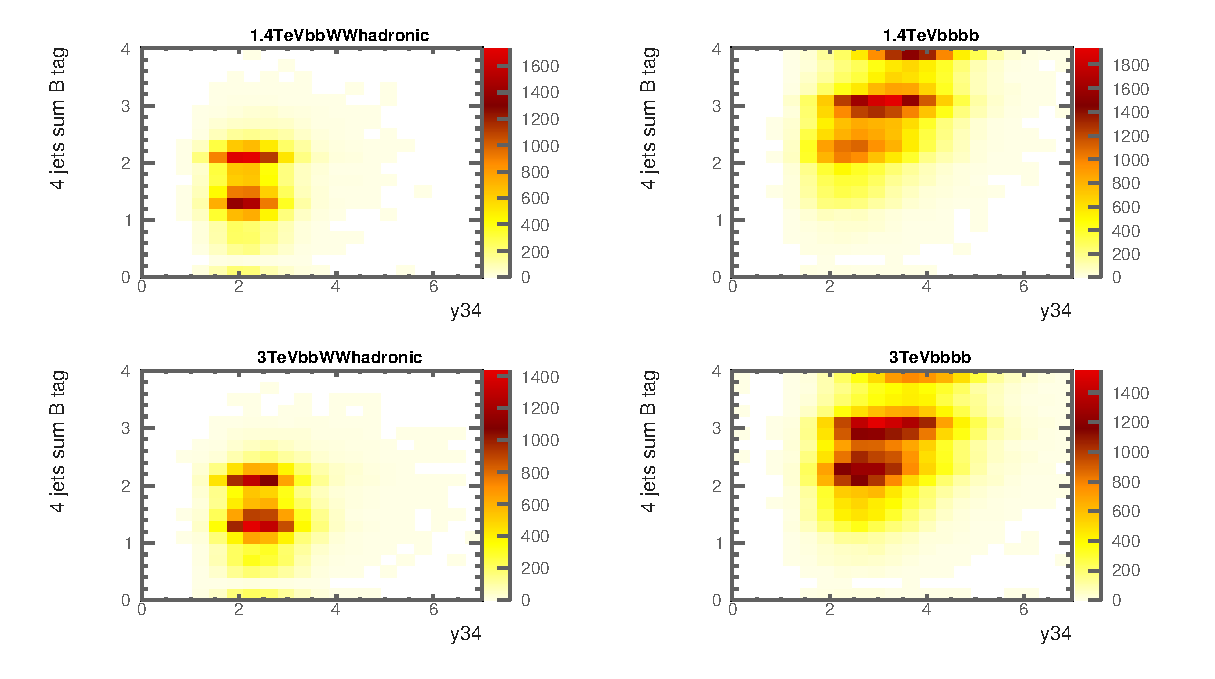
\includegraphics[width=\largefigwidth]{{doubleHiggs/sumbtagY34.eps}} \\

\caption[Sum of b tag against \y{34}]%
   {Sum of b tag against \y{34}, shown for signal samples}
   \label{fig:doubleHiggsMutualPreselection}
\end{figure}

\begin{table}[!tbp]\centering

\begin{tabular}{llrr}
\hline
\hline
\sqrtS & $selection$ & \multicolumn{1}{m{4cm}}{\eeToHHbbqqqq Selection Efficiency} & \multicolumn{1}{m{4cm}}{\eeToHHbbbb Selection Efficiency} \\
1.4\,TeV &  \sumBtag{4} < 2.3 and \y{34} < 3.7 & 86\% & 78\% \\
3\,TeV &  \sumBtag{4} < 2.3 and \y{34} < 3.6 & 89\% & 82\% \\
\hline
\hline
\end{tabular}
\caption[Mutually exclusive cuts] %
{Mutually exclusive cuts, for full signal samples}
\label{tab:doubleHiggsMutualCuts}
\end{table}

The selection efficiencies after mutually exclusive cuts and other pre-selection cuts stated above, are listed in \Table{}.

\begin{table}[!tbp]\centering
\small
\begin{tabular}{lrrrr}
\hline \hline
 \multicolumn{1}{m{3.5cm}}{Channel / Efficiency} &  \multicolumn{1}{m{2cm}}{Sanity \rootS{1.4}}  & \multicolumn{1}{m{2cm}}{Mutually exclusive \rootS{1.4}} & \multicolumn{1}{m{2cm}}{Sanity \rootS{3}} & \multicolumn{1}{m{2cm}}{Mutually exclusive \rootS{3}} \\
\hline
\eeToHH $\to$ \\
\HepProcess{ \Pbottom \APbottom \PWplus \PWminus \Pnu \APnu}, hadronic             & 66.4\%& 59.7\% & 69.5\% & 61.7\%\\
\hline
\eeToHH $\to$ \\
\HepProcess{ \Pbottom \APbottom \Pbottom \APbottom \Pnu \APnu}             &80.6\%& 15.4\% & 81.1\% & 18.8\% \\
\eeToHH $\to$ other & 24.7\% & 20.5\% & 25.1\% & 20.0\% \\
\hline
\eeTo{\qlight \qlight \PHiggs \Pnu \APnu}  & 42.0\% & 39.5\% & 40.3\% & 35.9\%\\
\eeTo{\Pcharm \APcharm \PHiggs \Pnu \APnu}  & 43.4\% & 31.7\%& 39.2\%& 26.2\%\\
\eeTo{\Pbottom \APbottom \PHiggs \Pnu \APnu}  & 64.2\% & 25.2\%& 64.2\%& 25.9\%\\

\eeTo{ \Pquark \Pquark \Pquark \Pquark}   & 4.6\%  & 3.4\% & 2.5\%& 1.4\%\\
\eeTo{ \Pquark \Pquark \Pquark \Pquark \Plepton \Plepton}& 3.3\% & 3.1\%& 0.7\%& 0.6\%\\
\eeTo{ \Pquark \Pquark \Pquark \Pquark \Plepton \Pnu}& 11.4\%. & 9.8\%& 9.2\%& 7.2\%\\
\eeTo{ \Pquark \Pquark \Pquark \Pquark \Pnu \APnu} & 18.8\% & 16.6\%& 11.8\%& 9.0\%\\

\eeTo{ \Pquark \Pquark} &  2.0\% & 0.8\%& 2.5\%& 1.4\%\\
\eeTo{ \Pquark \Pquark \Plepton \Pnu} &  1.6\% & 0.9\%& 0.3\%& 0.1\%\\
\eeTo{ \Pquark \Pquark \Pl \Pl} &  0.1\% & 0.1\%& 0.7\%& 0.4\%\\
\eeTo{ \Pquark \Pquark \Pnu \Pnu} & 5.8\% & 4.0\%& 5.3\%& 3.1\% \\
\hline
\egamma{\Pem}{\Pphoton}{BS}{\Pem \Pquark \Pquark \Pquark \Pquark} & 0.4\%  & 0.3\%& 0.8\%& 0.7\%\\
\egamma{\Pep}{\Pphoton}{BS}{\Pep \Pquark \Pquark \Pquark \Pquark} & 0.4\% & 0.4\%& 0.8\%& 0.7\%\\
\egamma{\Pem}{\Pphoton}{EPA}{\Pem \Pquark \Pquark \Pquark \Pquark} & 0.3\% & 0.2\%& 0.4\%& 0.4\%\\
\egamma{\Pep}{\Pphoton}{EPA}{\Pep \Pquark \Pquark \Pquark \Pquark}  & 0.3\% & 0.3\% & 0.4\%& 0.3\%\\
\egamma{\Pem}{\Pphoton}{BS}{\Pnu \Pquark \Pquark \Pquark \Pquark}& 27.7\%  & 25.3\%& 20.3\%& 16.8\%\\
\egamma{\Pep}{\Pphoton}{BS}{\APnu \Pquark \Pquark \Pquark \Pquark}& 27.3\% & 24.9\% & 19.3\%& 15.9\%\\
\egamma{\Pem}{\Pphoton}{EPA}{\Pnu \Pquark \Pquark \Pquark \Pquark}&  13.9\% & 12.6\% & 9.4\%& 7.8\%\\
\egamma{\Pep}{\Pphoton}{EPA}{\APnu \Pquark \Pquark \Pquark \Pquark}& 13.7\%  & 12.3\%& 8.9\%& 7.3\% \\

\egamma{\Pem}{\Pphoton}{BS}{\Pquark \Pquark \PHiggs \Pnu} & 34.6\%  & 30.6\% &37.2\%& 30.2\% \\
\egamma{\Pep}{\Pphoton}{BS}{\Pquark \Pquark \PHiggs \Pnu} & 34.6\% & 30.6\% & 37.1\% & 30.2\% \\
\egamma{\Pem}{\Pphoton}{EPA}{\Pquark \Pquark \PHiggs \Pnu} & 18.2\% & 16.0\% & 19.0\% & 15.7\% \\
\egamma{\Pep}{\Pphoton}{EPA}{\Pquark \Pquark \PHiggs \Pnu} & 18.4\%   & 16.1\% & 18.4\% & 15.2\% \\
\hline
\gammagamma{\Pphoton}{BS}{\Pphoton}{BS}{ \Pquark \Pquark \Pquark \Pquark}& 0.3\%  & 0.3\%& 1.9\%& 1.7\%\\
\gammagamma{\Pphoton}{BS}{\Pphoton}{EPA}{ \Pquark \Pquark \Pquark \Pquark}& 0.4\%  &0.3\%& 1.1\%& 1.0\%\\
\gammagamma{\Pphoton}{EPA}{\Pphoton}{BS}{ \Pquark \Pquark \Pquark \Pquark}& 0.4\% & 0.3\%& 1.1\%& 1.0\%\\
\gammagamma{\Pphoton}{EPA}{\Pphoton}{EPA}{ \Pquark \Pquark \Pquark \Pquark}& 0.4\% & 0.3\% & 0.7\% & 0.6\%\\
\hline \hline
\end{tabular}

\caption{List of signal and background samples with the corresponding expected number at \rootS{1.4} and \rootS{3}, assuming a luminosity of 1500 and 2000$fb^{-1}$, respectively. The selection efficiencies are presented in a ``flow'' fashion, as the every selection cut contains all the cuts to the left of it.
}
\label{tab:doubleHiggsPreslectionPart2}
\end{table}


\begin{comment}
    const TCut selectionCut3000 = "tR0_7_6jet_btag2_ChiSquared<20  && TightIsoLepTauAll_nPfo < 1 && BonoForwardElectronPhotons_nPfo < 1 && \
         tR0_7_6jet_btag2_Higgs_all_M>150  && \
       tR0_7_4jet_btag2_Higgs_all_bTag < 2.3 && tR0_7_6jet_btag2_minusLogY34 < 3.7 \
       && tR0_7_6jet_btag2_bTag1 > 0.7 &&\
        tR0_7_6jet_btag2_Higgs_all_M  < 3000 &&  tR0_7_6jet_btag2_Higgs1_M < 500 &&  tR0_7_6jet_btag2_Higgs2_M < 800 &&  tR0_7_6jet_btag2_W_Onshell_M < 200";

    const TCut selectionCut1400 = "nR0_7_6jet_btag2_ChiSquared<20  && IsoLepTauAll_nPfo < 1      && BonoForwardElectronPhotons_nPfo < 1 && nR0_7_6jet_btag2_Higgs_all_M>150 && \
        nR0_7_4jet_btag2_Higgs_all_bTag < 2.3  && nR0_7_6jet_btag2_minusLogY34 < 3.6 \
        &&  nR0_7_6jet_btag2_bTag2 > 0.2 && nR0_7_6jet_btag2_Higgs_all_Pt> 30 &&\
        nR0_7_6jet_btag2_Higgs_all_M  < 1400 &&  nR0_7_6jet_btag2_Higgs1_M < 500 &&  nR0_7_6jet_btag2_Higgs2_M < 800 &&  nR0_7_6jet_btag2_W_Onshell_M < 200";
\end{comment}

\section{Discriminative Variables}

A series of discriminative variables were calculated, and fed into MVA for signal selection.

The full list of variables can be found in \Table{}.
Same set of variables are used for \rootS{1.4} and \rootS{3}.

\Figure shows the the variable XX which gives a good discrimination of signal against background.

\begin{table}[!tbp]\centering
\begin{tabular}{ll}
\hline
\hline
 \multicolumn{1}{m{3cm}}{Variable} &  \multicolumn{1}{m{\widthOne}}{Description} \\
 \multicolumn{1}{m{3cm}}{$m_{\Hbb}$} &  \multicolumn{1}{m{0.7\textwidth}}{Invariant mass of \Hbb } \\
 \multicolumn{1}{m{3cm}}{$m_{\HWW}$} &  \multicolumn{1}{m{0.7\textwidth}}{Invariant mass of \HWW } \\
 \multicolumn{1}{m{3cm}}{$m_{\PW}$} &  \multicolumn{1}{m{10cm}}{Invariant mass of \PW } \\
 \multicolumn{1}{m{3cm}}{$m_{\HH}$} &  \multicolumn{1}{m{10cm}}{Invariant mass of \HH } \\
 \multicolumn{1}{m{3cm}}{$E_{\W*}$} &  \multicolumn{1}{m{10cm}}{Energy of \W* } \\
 \multicolumn{1}{m{3cm}}{$E_{mis}$} &  \multicolumn{1}{m{10cm}}{Missing energy, assuming collision at \sqrtS} \\
 \multicolumn{1}{m{3cm}}{$\pT_{\Hbb}$} &  \multicolumn{1}{m{10cm}}{Transverse momentum of \Hbb } \\
 \multicolumn{1}{m{3cm}}{$\pT_{\HWW}$} &  \multicolumn{1}{m{10cm}}{Transverse momentum of \HWW } \\
 \multicolumn{1}{m{3cm}}{$\pT_{\HH}$} &  \multicolumn{1}{m{10cm}}{Transverse momentum of \HH } \\
 \multicolumn{1}{m{3cm}}{$\eta_{mis}$} &  \multicolumn{1}{m{10cm}}{Pseudorapidity of missing momentum, assuming collision at \sqrtS} \\
 \multicolumn{1}{m{3cm}}{$\pT_{\HH}$} &  \multicolumn{1}{m{10cm}}{Transverse momentum of \HH } \\
 \multicolumn{1}{m{3cm}}{$-\ln(\y{23})$} &  \multicolumn{1}{m{10cm}}{minus ln of \y{23}. See \Section{} for \y{} parameter. See \Section{} for the ln transformation } \\
 \multicolumn{1}{m{3cm}}{$-\ln(\y{34})$} &  \multicolumn{1}{m{10cm}}{minus ln of \y{34}.} \\
 \multicolumn{1}{m{3cm}}{$-\ln(\y{45})$} &  \multicolumn{1}{m{10cm}}{minus ln of \y{45}.} \\
 \multicolumn{1}{m{3cm}}{$-\ln(\y{56})$} &  \multicolumn{1}{m{10cm}}{minus ln of \y{56}.} \\
 \multicolumn{1}{m{3cm}}{$\btagFull{1,\Hbb}$} &  \multicolumn{1}{m{10cm}}{Highest b-jet tag value of two jets forming \Hbb .} \\
 \multicolumn{1}{m{3cm}}{$\btagFull{2,\Hbb}$} &  \multicolumn{1}{m{10cm}}{Lowest b-jet tag value of two jets forming \Hbb .} \\
 \multicolumn{1}{m{3cm}}{$\btagFull{1,\PW}$} &  \multicolumn{1}{m{10cm}}{Highest b-jet tag value of two jets forming \PW .} \\
 \multicolumn{1}{m{3cm}}{$\btagFull{1,\W*}$} &  \multicolumn{1}{m{10cm}}{Highest b-jet tag value of two jets forming \W* .} \\
 \multicolumn{1}{m{3cm}}{$\ctagFull{1,\Hbb}$} &  \multicolumn{1}{m{10cm}}{Highest c-jet tag value of two jets forming \Hbb .} \\
 \multicolumn{1}{m{3cm}}{$\ctagFull{1,\PW}$} &  \multicolumn{1}{m{10cm}}{Highest c-jet tag value of two jets forming \PW .} \\
 \multicolumn{1}{m{3cm}}{$\abs{\sphericity}$} &  \multicolumn{1}{m{10cm}}{Modulus of sphericity, \sphericity. See \Section{}.} \\
 \multicolumn{1}{m{3cm}}{$\acolinearity{\Hbb}$} &  \multicolumn{1}{m{10cm}}{Acolinearity of two jets forming \Hbb.} \\
 \multicolumn{1}{m{3cm}}{$\acolinearity{\PW}$} &  \multicolumn{1}{m{10cm}}{Acolinearity of two jets forming \PW.} \\
 \multicolumn{1}{m{3cm}}{$\acolinearity{\HH}$} &  \multicolumn{1}{m{10cm}}{Acolinearity of \Hbb and \HWW.} \\
 \multicolumn{1}{m{3cm}}{$\npfo{\Hbb}$} &  \multicolumn{1}{m{10cm}}{Number of PFOs forming \Hbb.} \\
 \multicolumn{1}{m{3cm}}{$\npfo{\HWW}$} &  \multicolumn{1}{m{10cm}}{Number of PFOs forming \HWW.} \\
 \multicolumn{1}{m{3cm}}{$\npfo{\PW}$} &  \multicolumn{1}{m{10cm}}{Number of PFOs forming \PW.} \\
 \multicolumn{1}{m{3cm}}{$\npfo{\W*}$} &  \multicolumn{1}{m{10cm}}{Number of PFOs forming \W*.} \\
 \multicolumn{1}{m{3cm}}{$\cosStar{\Hbb}$} &  \multicolumn{1}{m{10cm}}{Cosine of opening angles of two jets forming \Hbb, in their rest frame.} \\
 \multicolumn{1}{m{3cm}}{$\cosStar{\HWW}$} &  \multicolumn{1}{m{10cm}}{Cosine of opening angles of \PW and \W*, forming \HWW, in their rest frame.} \\
 \multicolumn{1}{m{3cm}}{$\cosStar{\PW}$} &  \multicolumn{1}{m{10cm}}{Cosine of opening angles of two jets forming \PW, in their rest frame.} \\
 \multicolumn{1}{m{3cm}}{$\cosStar{\W*}$} &  \multicolumn{1}{m{10cm}}{Cosine of opening angles of two jets forming \W*, in their rest frame.} \\
 \multicolumn{1}{m{3cm}}{$\cosStar{\HH}$} &  \multicolumn{1}{m{10cm}}{Cosine of opening angles of \Hbb and \HWW, in their rest frame.} \\
\hline
\hline
\end{tabular}
\caption[List of variables used in MVA] %
{List of variables used in MVA}
\label{tab:doubleHiggsVaraibles}
\end{table}

The optimal set were chosen to give the best MVA performance, whilst no strong pair-wise correlation between any two variables, shown in \Figure{}.



\section{Multivariate analysis}

Multivariate analysis was performed with TMVA package. The classifier that performs the best was found to be the boosted decision tree. See \Section{} for details on boosted decision tree.

The parameters for boosted decision tree were optimised and checked for overtraining. The most important variables are the depth of the tree and the number of trees. Other parameters includes the minimum number of nodes in a leaf, the number of cuts of a variable, the learning rate, the sampling fraction, the yes/no or purity leaf, adaBoost or gradient boost.

The optimisation and overtraining test was done with \rootS{3} samples. \rootS{1.4} samples produce similar results.

Half of the samples were used for training, and the other half used for testing.

% TODO discuss BDT TMVA first, then come back here
% TODO discuss each variables

\section{Signal selection results}

\begin{table}[!tbp]\centering
%\small{
\small
\begin{tabular}{lrrrr}
\hline \hline
 \multicolumn{1}{m{3.5cm}}{Channel / Efficiency \rootS{1.4}} &  \multicolumn{1}{m{2cm}}{Expected number of events}  & \multicolumn{1}{m{2cm}}{Pre-selection efficiency} & \multicolumn{1}{m{2cm}}{MVA efficiency} & \multicolumn{1}{m{2cm}}{Number of events after MVA} \\
\hline
\eeToHH $\to$ \\
\HepProcess{ \Pbottom \APbottom \PWplus \PWminus \Pnu \APnu}, hadronic             &27.9& 59.8\% & 8.2\% & 1.37 \\
\hline
\eeToHH $\to$ \\
\HepProcess{ \Pbottom \APbottom \Pbottom \APbottom \Pnu \APnu}             &67.6& 15.4\%  & 0.5\% & 0.05\\
\eeToHH $\to$ other                             & 128.0 & 20.4\% & 1.7\% & 0.45\\
\hline
\eeTo{\qlight \qlight \PHiggs \Pnu \APnu}  & 1304.0 & 39.5\% & 0.05\%& 0.29\\
\eeTo{\Pcharm \APcharm \PHiggs \Pnu \APnu}  & 546.1 & 31.6\%& 0.1\%& 0.16\\
\eeTo{\Pbottom \APbottom \PHiggs \Pnu \APnu}  & 463.0 & 24.7\%& 0.3\%& 0.37\\

\eeTo{ \Pquark \Pquark \Pquark \Pquark}   &   1867650.0& 3.3\% & - & -\\
\eeTo{ \Pquark \Pquark \Pquark \Pquark \Plepton \Plepton}& 93150.0 & 0.3\%& - &  - \\
\eeTo{ \Pquark \Pquark \Pquark \Pquark \Plepton \Pnu}& 165600.0 & 9.8\%& 0.01\%& 2.06\\
\eeTo{ \Pquark \Pquark \Pquark \Pquark \Pnu \APnu} & 34800.0& 16.5\%& 0.002\% & 0.10\\

\eeTo{ \Pquark \Pquark} &  6014250.0 & 0.8\%& - & - \\
\eeTo{ \Pquark \Pquark \Plepton \Pnu} &  6464550.0 & 0.9\%&  - & - \\
\eeTo{ \Pquark \Pquark \Pl \Pl} &  4088700.0 & 0.08\%& - & - \\
\eeTo{ \Pquark \Pquark \Pnu \Pnu} & 1181550.0 & 4.0\%& - & - \\
\hline
\egamma{\Pem}{\Pphoton}{BS}{\Pem \Pquark \Pquark \Pquark \Pquark} & 1305787.5  & 0.3\%& - & -\\
\egamma{\Pep}{\Pphoton}{BS}{\Pep \Pquark \Pquark \Pquark \Pquark} & 1300837.5 & 0.4\%& -& -\\
\egamma{\Pem}{\Pphoton}{EPA}{\Pem \Pquark \Pquark \Pquark \Pquark} & 430650.0 & 0.3\%&  - &  - \\
\egamma{\Pep}{\Pphoton}{EPA}{\Pep \Pquark \Pquark \Pquark \Pquark}  & 430350.0 & 0.3\% & - & -\\
\egamma{\Pem}{\Pphoton}{BS}{\Pnu \Pquark \Pquark \Pquark \Pquark}& 89775.0  & 25.4\%& 0.005\%& 1.09\\
\egamma{\Pep}{\Pphoton}{BS}{\APnu \Pquark \Pquark \Pquark \Pquark}& 89212.5 & 24.9\% & 0.004\%& 0.96\\
\egamma{\Pem}{\Pphoton}{EPA}{\Pnu \Pquark \Pquark \Pquark \Pquark}& 26100.0  & 12.6\% & - &  - \\
\egamma{\Pep}{\Pphoton}{EPA}{\APnu \Pquark \Pquark \Pquark \Pquark}& 25950.0  & 12.4\%& 0.008\% & 0.27\\

\egamma{\Pem}{\Pphoton}{BS}{\Pquark \Pquark \PHiggs \Pnu} & 17775   & 30.8\% & 0.02\% & 1.00 \\
\egamma{\Pep}{\Pphoton}{BS}{\Pquark \Pquark \PHiggs \Pnu} & 17662.5  & 30.6\% & 0.02\% & 1.16 \\
\egamma{\Pem}{\Pphoton}{EPA}{\Pquark \Pquark \PHiggs \Pnu} & 5085  & 16.0\% & 0.04\% & 0.33 \\
\egamma{\Pep}{\Pphoton}{EPA}{\Pquark \Pquark \PHiggs \Pnu} & 5085   & 16.2\% & 0.08\% & 0.62 \\
\hline
\gammagamma{\Pphoton}{BS}{\Pphoton}{BS}{ \Pquark \Pquark \Pquark \Pquark}& 2054951.5  & 0.2\%&  - & -\\
\gammagamma{\Pphoton}{BS}{\Pphoton}{EPA}{ \Pquark \Pquark \Pquark \Pquark}& 4521037.5  & 0.4\%& - & - \\
\gammagamma{\Pphoton}{EPA}{\Pphoton}{BS}{ \Pquark \Pquark \Pquark \Pquark}& 4539150.0 & 0.3\%&  - & - \\
\gammagamma{\Pphoton}{EPA}{\Pphoton}{EPA}{ \Pquark \Pquark \Pquark \Pquark}& 1129500.0 & 0.3\% & - & -\\
\hline \hline
\end{tabular}

\caption{List of signal and background samples with the corresponding expected number at  \rootS{1.4}, for a luminosity of 1500$fb^{-1}$. The number of events, selection efficiency of pre-selection, selection efficiency of MVA after pre-selection, number of events after MVA are shown. - represents no events passing the MVA.
}
\label{tab:doubleHiggs1.4TeVMVA}
\end{table}

\begin{table}[!tbp]\centering
%\small{
\small
\begin{tabular}{lrrrr}
\hline \hline
 \multicolumn{1}{m{3.5cm}}{Channel / Efficiency \rootS{3}} &  \multicolumn{1}{m{2cm}}{Expected number of events}  & \multicolumn{1}{m{2cm}}{Pre-selection efficiency} & \multicolumn{1}{m{2cm}}{MVA efficiency} & \multicolumn{1}{m{2cm}}{Number of events after MVA} \\
\hline
\eeToHH $\to$ \\
\HepProcess{ \Pbottom \APbottom \PWplus \PWminus \Pnu \APnu}, hadronic             &146.0& 61.7\% & 11.6\% & 10.43\\
\hline
\eeToHH $\to$ \\
\HepProcess{ \Pbottom \APbottom \Pbottom \APbottom \Pnu \APnu}             &355.0& 18.8\% & 1.5\% & 1.01 \\
\eeToHH $\to$ other                             & 675.0 & 20.0\% & 3.6\% & 4.93 \\
\hline
\eeTo{\qlight \qlight \PHiggs \Pnu \APnu}  & 6115.4 & 36.0\% & 0.4\% & 9.42\\
\eeTo{\Pcharm \APcharm \PHiggs \Pnu \APnu}  & 2249.9 & 26.3\%& 0.5\%& 3.13\\
\eeTo{\Pbottom \APbottom \PHiggs \Pnu \APnu}  & 2197.7 & 25.8\%& 1.2\%& 6.82\\

\eeTo{ \Pquark \Pquark \Pquark \Pquark}   &   1093000.0& 1.4\% & 0.01\%& 1.43\\
\eeTo{ \Pquark \Pquark \Pquark \Pquark \Plepton \Plepton}& 338600.0 & 0.6\%&  - & -\\
\eeTo{ \Pquark \Pquark \Pquark \Pquark \Plepton \Pnu}& 213200.0 & 7.3\%& 0.05\%& 8.35\\
\eeTo{ \Pquark \Pquark \Pquark \Pquark \Pnu \APnu} & 143000.0& 9.0\%& 0.05\%& 6.35\\

\eeTo{ \Pquark \Pquark} &  5897800.0 & 1.4\%&  - & - \\
\eeTo{ \Pquark \Pquark \Plepton \Pnu} &  11121800 & 0.1\%& - & - \\
\eeTo{ \Pquark \Pquark \Pl \Pl} &  6639200.0 & 0.4\%& - & - \\
\eeTo{ \Pquark \Pquark \Pnu \Pnu} & 2635000.0 & 3.1\%&  - & - \\
\hline
\egamma{\Pem}{\Pphoton}{BS}{\Pem \Pquark \Pquark \Pquark \Pquark} & 2004388.1  & 0.7\%&  - & - \\
\egamma{\Pep}{\Pphoton}{BS}{\Pep \Pquark \Pquark \Pquark \Pquark} & 2002334.1 & 0.7\%&  - & - \\
\egamma{\Pem}{\Pphoton}{EPA}{\Pem \Pquark \Pquark \Pquark \Pquark} & 575600.0& 0.4\%&  - & - \\
\egamma{\Pep}{\Pphoton}{EPA}{\Pep \Pquark \Pquark \Pquark \Pquark}  & 575600.0 & 0.3\% &  - & - \\

\egamma{\Pem}{\Pphoton}{BS}{\Pnu \Pquark \Pquark \Pquark \Pquark}& 414750.0  & 16.8\%& 0.04\%& 30.7\\
\egamma{\Pep}{\Pphoton}{BS}{\APnu \Pquark \Pquark \Pquark \Pquark}& 414434.0 & 15.9\% & 0.05\%& 30.3\\
\egamma{\Pem}{\Pphoton}{EPA}{\Pnu \Pquark \Pquark \Pquark \Pquark}& 108400.0  & 7.8\% & 0.04\%& 3.37\\
\egamma{\Pep}{\Pphoton}{EPA}{\APnu \Pquark \Pquark \Pquark \Pquark}& 108400.0  & 7.3\%& 0.03\%& 2.63 \\

\egamma{\Pem}{\Pphoton}{BS}{\Pquark \Pquark \PHiggs \Pnu} & 92588.0  & 30.2\% & 0.2\%& 67.5 \\
\egamma{\Pep}{\Pphoton}{BS}{\Pquark \Pquark \PHiggs \Pnu} & 92430.0 & 30.3\% & 0.2\% & 54.2 \\
\egamma{\Pem}{\Pphoton}{EPA}{\Pquark \Pquark \PHiggs \Pnu} & 23400.0 & 15.4\% & 0.2\% & 7.88 \\
\egamma{\Pep}{\Pphoton}{EPA}{\Pquark \Pquark \PHiggs \Pnu} & 23400.0   & 15.2\% & 0.3\% & 10.2 \\
\hline
\gammagamma{\Pphoton}{BS}{\Pphoton}{BS}{ \Pquark \Pquark \Pquark \Pquark}& 18009413.9  & 1.6\%&   - & - \\
\gammagamma{\Pphoton}{BS}{\Pphoton}{EPA}{ \Pquark \Pquark \Pquark \Pquark}& 3824548.1  & 1.0\%&  - & - \\
\gammagamma{\Pphoton}{EPA}{\Pphoton}{BS}{ \Pquark \Pquark \Pquark \Pquark}& 3828498.1 & 1.0\%&  - & - \\
\gammagamma{\Pphoton}{EPA}{\Pphoton}{EPA}{ \Pquark \Pquark \Pquark \Pquark}& 805400.0 & 0.6\%&  - & - \\
\hline \hline
\end{tabular}
\caption{List of signal and background samples with the corresponding expected number at  \rootS{3}, for a luminosity of 2000$fb^{-1}$. The number of events, selection efficiency of pre-selection, selection efficiency of MVA after pre-selection, number of events after MVA are shown. - represents no events passing the MVA.
}
\label{tab:doubleHiggs3TeVMVA}
\end{table}


\begin{table}[!tbp]\centering
%\small{
\small
\begin{tabular}{lrrrr}
\hline \hline
 \multicolumn{1}{m{3.5cm}}{Channel / Efficiency \rootS{3}} &  \multicolumn{1}{m{2cm}}{Expected number of events}  & \multicolumn{1}{m{2cm}}{Pre-selection efficiency} & \multicolumn{1}{m{2cm}}{MVA efficiency} & \multicolumn{1}{m{2cm}}{Number of events after MVA} \\
\hline
\eeToHH $\to$ \\
\HepProcess{ \Pbottom \APbottom \PWplus \PWminus \Pnu \APnu}, semi-leptonic       &96.8& 44.6\% & 21.9\% & 9.48\\
\hline
\eeToHH $\to$ \\
\HepProcess{ \Pbottom \APbottom \Pbottom \APbottom \Pnu \APnu}             &355.0& 13.3\% & 10.9\% &  5.16\\
\eeToHH $\to$ other                             & 724.2 & 13.1\% & 13.6\% &  12.89\\
\hline
\eeTo{\qlight \qlight \PHiggs \Pnu \APnu}  & 6115.4 & 7.4\% & 13.7\% & 62.63\\
\eeTo{\Pcharm \APcharm \PHiggs \Pnu \APnu}  & 2249.9 & 6.3\%& 12.1\%& 17.10\\
\eeTo{\Pbottom \APbottom \PHiggs \Pnu \APnu}  & 2197.7 & 15.9\%& 5.1\%& 18.03\\

\eeTo{ \Pquark \Pquark \Pquark \Pquark}   &   1093000.0& 0.6\% & 0.2\%& 15.04\\
\eeTo{ \Pquark \Pquark \Pquark \Pquark \Plepton \Plepton}& 338600.0 & 1.0\%&  0.06\% & 1.85\\
\eeTo{ \Pquark \Pquark \Pquark \Pquark \Plepton \Pnu}& 213200.0 & 27.6\%& 0.5\%& 270.33\\
\eeTo{ \Pquark \Pquark \Pquark \Pquark \Pnu \APnu} & 143000.0& 1.9\%& 1.6\%& 43.78\\

\eeTo{ \Pquark \Pquark} &  5897800.0 & 0.4\%&  0.3\% & 60.82 \\
\eeTo{ \Pquark \Pquark \Plepton \Pnu} &  11121800 & 0.3\%& 0.08\% & 21.24 \\
\eeTo{ \Pquark \Pquark \Pl \Pl} &  6639200.0 & 0.6\%& 0.2\%& 84.14\\
\eeTo{ \Pquark \Pquark \Pnu \Pnu} & 2635000.0 & 0.4\%&  0.9\% & 92.55 \\
\hline
\egamma{\Pem}{\Pphoton}{BS}{\Pem \Pquark \Pquark \Pquark \Pquark} & 2004388.1  & 1.2\%&  - & - \\
\egamma{\Pep}{\Pphoton}{BS}{\Pep \Pquark \Pquark \Pquark \Pquark} & 2002334.1 & 1.2\%&  - & - \\
\egamma{\Pem}{\Pphoton}{EPA}{\Pem \Pquark \Pquark \Pquark \Pquark} & 575600.0& 1.1\%&  - & - \\
\egamma{\Pep}{\Pphoton}{EPA}{\Pep \Pquark \Pquark \Pquark \Pquark}  & 575600.0 & 1.1\% &  - & - \\

\egamma{\Pem}{\Pphoton}{BS}{\Pnu \Pquark \Pquark \Pquark \Pquark}& 414750.0  & 3.7\%& 1.5\%& 226.77\\
\egamma{\Pep}{\Pphoton}{BS}{\APnu \Pquark \Pquark \Pquark \Pquark}& 414434.0 & 3.5\% & 1.6\%& 225.68\\
\egamma{\Pem}{\Pphoton}{EPA}{\Pnu \Pquark \Pquark \Pquark \Pquark}& 108400.0  & 11.2\% & 0.9\%& 107.90\\
\egamma{\Pep}{\Pphoton}{EPA}{\APnu \Pquark \Pquark \Pquark \Pquark}& 108400.0  & 10.7\%& 0.8\%& 92.75 \\

\egamma{\Pem}{\Pphoton}{BS}{\Pquark \Pquark \PHiggs \Pnu} & 92588.0  & 7.9\% & 10.7\%& 779.36 \\
\egamma{\Pep}{\Pphoton}{BS}{\Pquark \Pquark \PHiggs \Pnu} & 92430.0 & 7.9\% & 10.1\% & 741.57 \\
\egamma{\Pem}{\Pphoton}{EPA}{\Pquark \Pquark \PHiggs \Pnu} & 23400.0 & 22.9\% & 6.9\% & 369.52 \\
\egamma{\Pep}{\Pphoton}{EPA}{\Pquark \Pquark \PHiggs \Pnu} & 23400.0   & 22.7\% & 7.2\% & 381.33 \\
\hline
\gammagamma{\Pphoton}{BS}{\Pphoton}{BS}{ \Pquark \Pquark \Pquark \Pquark}& 18009413.9  & 0.4\%&   - & - \\
\gammagamma{\Pphoton}{BS}{\Pphoton}{EPA}{ \Pquark \Pquark \Pquark \Pquark}& 3824548.1  & 1.0\%&  - & - \\
\gammagamma{\Pphoton}{EPA}{\Pphoton}{BS}{ \Pquark \Pquark \Pquark \Pquark}& 3828498.1 & 1.0\%&  0.08\% & 28.85 \\
\gammagamma{\Pphoton}{EPA}{\Pphoton}{EPA}{ \Pquark \Pquark \Pquark \Pquark}& 805400.0 & 1.1\%&  - & - \\
\hline \hline
\end{tabular}
\caption{List of signal and background samples with the corresponding expected number at  \rootS{3}, for a luminosity of 2000$fb^{-1}$. The number of events, selection efficiency of pre-selection, selection efficiency of MVA after pre-selection, number of events after MVA are shown. - represents no events passing the MVA.
}
\label{tab:doubleHiggsQlv3TeVMVA}
\end{table}


\section{3\,TeV hadronic decay analysis}

The lepton finding processors are either developed or optimised with samples at \rootS{1.4}, and checked against samples at \rootS{3}. Because the expected signal significance would be low, the processors are optimised to aggressively reject more background, to increase the final signal significance. It was found that the same set of parameters for lepton identifiers work well under \rootS{1.4} and 3\,TeV.

Comparing \rootS{1.4} and \rootS{3}, the performance is worse for \rootS{3}. This is because particles are more boosted and separation because particles are smaller. This reflects on the performance of the  ForwardFinderProcessor. Whilst at \rootS{1.4}, the processor only rejects 5\% background and 1\% signal, at \rootS{3} it rejects 19\% background and 4\% signal, suggesting many leptons are in the forward region. These processors are complimentary and a good rejection rate with combined processors is achieved.

\begin{table}[!tbp]\centering
% TODO fix lumi correction for e gamma, gamma e
% TODO change some of sample cross section for  electron-photon interaction with four quarks and a neutrino final state
\small
%{

\begin{tabular}{lrr}
\hline \hline
Channel  &  $\sigma(\rootS{1.4})$ / fb  & $\sigma(\rootS{3})$ / fb   \\
\hline
\eeToHH & 0.149 &0.588 \\
\hline
\eeToHHbbWWFull,hadronic & 0.018 &0.07 \\
\eeToHHbbbbFull & 0.047 &0.19 \\
\eeToHHotherFull & 0.085 &0.34 \\
\hline
\eeTo{\qlight \qlight \PHiggs \Pnu \APnu}  & 0.86 & 1.78 \\
\eeTo{\Pcharm \APcharm \PHiggs \Pnu \APnu}  & 0.36 & 1.12\\
\eeTo{\Pbottom \APbottom \PHiggs \Pnu \APnu}  & 0.31 & 1.91\\

\eeTo{ \Pquark \Pquark \Pquark \Pquark}   &   1245.1& 546.5*\\
\eeTo{ \Pquark \Pquark \Pquark \Pquark \Plepton \Plepton}& 62.1* &169.3*\\
\eeTo{ \Pquark \Pquark \Pquark \Pquark \Plepton \Pnu}& 110.4* &106.6*\\
\eeTo{ \Pquark \Pquark \Pquark \Pquark \Pnu \APnu} & 23.2* &71.5*\\

\eeTo{ \Pquark \Pquark} &  4009.5 &2948.9\\
\eeTo{ \Pquark \Pquark \Plepton \Pnu} &  4309.7 &5561.1\\
\eeTo{ \Pquark \Pquark \Pl \Pl} &  2725.8 &3319.6\\
\eeTo{ \Pquark \Pquark \Pnu \Pnu} & 787.7 &1317.5 \\
\hline
\egamma{\Pem}{\Pphoton}{BS}{\Pem \Pquark \Pquark \Pquark \Pquark} & 1160.7  & 1268.7*\\
\egamma{\Pep}{\Pphoton}{BS}{\Pep \Pquark \Pquark \Pquark \Pquark} & 1156.3 & 1267.6*\\
\egamma{\Pem}{\Pphoton}{EPA}{\Pem \Pquark \Pquark \Pquark \Pquark} & 287.1 & 287.9*\\
\egamma{\Pep}{\Pphoton}{EPA}{\Pep \Pquark \Pquark \Pquark \Pquark}  & 286.9 & 287.8*\\
\egamma{\Pem}{\Pphoton}{BS}{\Pnu \Pquark \Pquark \Pquark \Pquark}& 79.8\myDagger  & 262.5*\\
\egamma{\Pep}{\Pphoton}{BS}{\APnu \Pquark \Pquark \Pquark \Pquark}& 79.3\myDagger & 262.3*\\
\egamma{\Pem}{\Pphoton}{EPA}{\Pnu \Pquark \Pquark \Pquark \Pquark}& 17.4\myDagger  & 54.2*\\
\egamma{\Pep}{\Pphoton}{EPA}{\APnu \Pquark \Pquark \Pquark \Pquark}& 17.3\myDagger  & 54.2*\\

\egamma{\Pem}{\Pphoton}{BS}{\Pquark \Pquark \PHiggs \Pnu} & 15.8*  & 58.6* \\
\egamma{\Pep}{\Pphoton}{BS}{\Pquark \Pquark \PHiggs \Pnu} & 15.7* & 58.5* \\
\egamma{\Pem}{\Pphoton}{EPA}{\Pquark \Pquark \PHiggs \Pnu} & 3.39*  & 11.7* \\
\egamma{\Pep}{\Pphoton}{EPA}{\Pquark \Pquark \PHiggs \Pnu} & 3.39*   & 11.7* \\
\hline
\gammagamma{\Pphoton}{BS}{\Pphoton}{BS}{ \Pquark \Pquark \Pquark \Pquark}& 21406.2*  &13050.3*\\
\gammagamma{\Pphoton}{BS}{\Pphoton}{EPA}{ \Pquark \Pquark \Pquark \Pquark}& 4018.7*  &2420.6*\\
\gammagamma{\Pphoton}{EPA}{\Pphoton}{BS}{ \Pquark \Pquark \Pquark \Pquark}& 4034.8* &2423.1*\\
\gammagamma{\Pphoton}{EPA}{\Pphoton}{EPA}{ \Pquark \Pquark \Pquark \Pquark}& 753.0* &402.7* \\
\hline \hline
\end{tabular}

\caption[]{List of signal and background samples with the corresponding cross sections at \rootS{3} and \rootS{1.4}. \Pquark can \Pup, \Pdown, \Pstrange, \Pbottom or \Ptop. Unless specified, \Pquark, \Plepton and \Pnu represent particles and its corresponding anti-particles. \Pphoton(BS) represents a real photon from beamstrahlung (BS). \Pphoton(EPA) represents a ``quasi-real'' photon, simulated with the Equivalent Photon Approximation. For processes involving Higgs production explicitly, simulated Higgs mass is 126\,GeV. Otherwise, Higgs mass is set to 14\,TeV. For processes labeled with * and $\myDagger$, the generator level cut requires invariant mass of quarks greater than 50 and 120\,GeV, respectively.}
\label{tab:samples_xsec}
\end{table}


\begin{table}[!tbp]
\begin{tabular}{lrr}
\hline
\hline
Efficiency (1.4\,TeV)  &  Signal & \HepProcess{\Pep \Pem \to \Pquark\Pquark\Pquark\Pquark\Plepton\Pnu} \\
\hline
IsolatedLeptonFinderProcessor & 99.3\% & 50.3\%  \\
BonoLeptonFinderProcessor & 99.1\% & 39.9\%  \\
TauFinderProcessor & 97.5\% & 52.3\%  \\
BonoTauFinderProcessor & 89.7\% & 38.5\%  \\
ForwardFinderProcessor & 98.9\% & 95.1\%  \\
Combined & 86.6\% & 16.8\%  \\
\hline
Efficiency (3\,TeV)  &  Signal  & \HepProcess{\Pep \Pem \to \Pquark\Pquark\Pquark\Pquark\Plepton\Pnu} \\
\hline
IsolatedLeptonFinderProcessor & 99.5\% & 66.8\%  \\
BonoLeptonFinderProcessor & 99.0\% & 52.5\%  \\
TauFinderProcessor & 97.7\% & 79.5\%  \\
BonoTauFinderProcessor & 86.3\% & 60.3\%  \\
ForwardFinderProcessor & 95.9\% & 80.7\%  \\
Combined & 81.0\% & 23.3\%  \\
\hline
\hline

\end{tabular}
\caption{isolated lepton finder processors performance on the signal and selected background samples.}
\label{tab:doubleHiggs3TeVIsoLepPerformance}
\end{table}

\begin{table}[!tbp]
\begin{tabular}{lrr}
\hline
\hline
Selection / Efficiency (1.4\,TeV)  &  Signal & \egamma{\Pem}{\Pphoton}{BS}{\Pem \Pquark \Pquark \Pquark \Pquark}  \\
\hline
Combined light lepton finder & 87.6\% & 67.5\%  \\
ForwardFinderProcessor & 98.9\% & 53.6\%  \\
Combined & 86.6\% & 30.8\%  \\
\hline
Processor / Efficiency (3\,TeV)  &  Signal  & \egamma{\Pem}{\Pphoton}{BS}{\Pem \Pquark \Pquark \Pquark \Pquark}  \\
\hline
Combined light lepton finder & 84.4\% & 72.7\%  \\
ForwardFinderProcessor & 95.9\% & 55.4\%  \\
Combined & 81.0\% &  33.4\%  \\
\hline
\hline

\end{tabular}
\caption{Very forward electron and photon finder performance on the signal and selected background samples.}
\label{tab:doubleHiggs3TeVForwardPerformance}
\end{table}
\section{Couplings extration} 